\documentclass[UTF8,a4paper,12pt]{ctexart}

% =========================================================
% 基础宏包
% =========================================================
\usepackage{geometry}
\usepackage{graphicx}
\usepackage{float}
\usepackage{booktabs}
\usepackage{array}
\usepackage{multirow}
\usepackage{amsmath, amssymb}
\usepackage{caption}
\usepackage{subcaption}
\usepackage{hyperref}
\usepackage{xcolor}
\usepackage{longtable}
\usepackage{tabularx}
\usepackage{setspace}
\usepackage{makecell}
\usepackage{xeCJK}
\geometry{left=2.6cm,right=2.6cm,top=2.5cm,bottom=2.5cm}
\setstretch{1.35}

\hypersetup{
    colorlinks=true,
    linkcolor=blue,
    citecolor=blue,
    urlcolor=blue
}

% =========================================================
% 表格设置
% =========================================================
\renewcommand\arraystretch{1.25}
\setlength{\tabcolsep}{5pt}

% =========================================================
% 图片占位命令
% 后续需要放图片时，把 \placeholderfig 替换成 includegraphics 即可
% =========================================================
\newcommand{\placeholderfig}[3][0.85\textwidth]{
\begin{figure}[H]
    \centering
    \fbox{
        \begin{minipage}[c][5cm][c]{#1}
            \centering
            \vspace{1.5cm}
            \textcolor{gray}{此处预留图片位置：#2}\\
            \textcolor{gray}{后续可替换为 \textbackslash includegraphics}
            \vspace{1.5cm}
        \end{minipage}
    }
    \caption{#2}
    \label{#3}
\end{figure}
}

% =========================================================
% 文档开始
% =========================================================
\begin{document}

\begin{titlepage}
    \centering
    \vspace*{2.5cm}
    {\zihao{2}\bfseries 人工智能基础课程设计\par}
    \vspace{2cm}
    {\zihao{1}\bfseries 基于 CIFAR-10 的对抗样本迁移攻击与鲁棒防御实验\par}
    \vspace{2.4cm}
    {\zihao{4}
    \renewcommand{\arraystretch}{1.7}
    \begin{tabular}{p{3.2cm}p{10.2cm}}
        题目： & 基于 CIFAR-10 的对抗样本迁移攻击与鲁棒防御实验 \\
        组员姓名学号： & 金纪勇\quad 2023141480172 \\
         & 周杨\quad 2023141490212 \\
         & 程湜\quad 2023141410200 \\
         & 廖苒希\quad 2024141450161 \\
         & 朱子淼\quad 2024141450073 \\
        日期： & 2026 年 7 月 9 日 \\
    \end{tabular}\par}
    \vfill
\end{titlepage}

\setcounter{page}{1}

\begin{abstract}
本文基于 CIFAR-10 构建 ResNet18 与 SimpleCNN 两个分类模型，对 FGSM、PGD、DeepFool、MI-FGSM 和 SPSA 攻击，以及 JPEG 压缩、位深压缩、FGSM/PGD 对抗训练进行系统比较。结果表明，白盒 PGD 攻击最强，MI-FGSM 迁移性最好，输入预处理防御在 BPDA 自适应攻击下容易失效，而 PGD 对抗训练具有最佳综合鲁棒性。
\end{abstract}

\noindent\textbf{关键词：} 对抗样本；迁移攻击；白盒攻击；黑盒攻击；PGD；对抗训练；BPDA；CIFAR-10

% % =========================================================
\section{引言}
% =========================================================

\subsection{项目背景}

近年来，深度学习技术在计算机视觉、自然语言处理、语音识别和自动驾驶等领域取得了显著进展。其中，卷积神经网络和 Transformer 等深度模型已经能够在图像分类任务中达到较高的准确率，并被广泛应用于人脸识别、智能安防、医学图像分析和无人驾驶感知等实际场景。然而，随着人工智能系统应用范围不断扩大，模型的安全性和可靠性问题也逐渐受到关注。

研究表明，深度神经网络虽然在干净样本上具有较强的分类能力，但对输入中的微小扰动十分敏感。攻击者可以在人眼几乎无法察觉的范围内对图像进行修改，使模型产生错误分类，这类经过特殊构造的样本被称为对抗样本。对抗样本的存在说明，深度学习模型学习到的决策边界并不总是与人类视觉感知保持一致，模型可能依赖一些脆弱的、非鲁棒的特征完成分类任务。

以图像分类任务为例，一张原本能够被正确识别为 cat、truck 或 airplane 的 CIFAR-10 图像，在加入幅度很小的扰动后，模型可能会将其错误分类为 dog、bird 或 automobile。虽然这种扰动对人眼来说几乎不可见，但对于深度神经网络而言，却可能导致输出结果发生明显变化。这种现象对人工智能系统的安全部署构成了潜在威胁，尤其是在自动驾驶、身份认证、智能监控等高安全性要求场景中，模型一旦被对抗样本误导，可能造成严重后果。

根据攻击者掌握目标模型信息的不同，对抗攻击通常可以分为白盒攻击、黑盒攻击和迁移攻击。白盒攻击假设攻击者能够完全获取目标模型的结构、参数和梯度信息，因此攻击能力最强；黑盒攻击假设攻击者无法获取模型内部信息，只能通过查询模型输出结果进行攻击，更接近真实应用环境；迁移攻击则利用对抗样本在不同模型之间可能具有迁移性的特点，先在一个已知源模型上生成对抗样本，再将其迁移到未知目标模型上进行攻击。

在实际场景中，攻击者往往难以直接获得目标模型的内部结构和参数，因此迁移攻击具有重要研究价值。若某一模型上生成的对抗样本能够成功攻击另一个模型，则说明不同模型之间可能共享某些相似的非鲁棒特征。这不仅揭示了深度模型决策机制中的共性问题，也说明仅依靠隐藏模型结构并不能完全保证系统安全。

因此，研究对抗样本攻击与防御方法，不仅有助于理解深度神经网络的脆弱性，也有助于设计更加稳定、可靠和安全的人工智能系统。本课程设计正是在这一背景下，基于 CIFAR-10 图像分类任务，系统实现并比较多种对抗攻击与防御方法，重点分析迁移攻击效果和鲁棒防御策略。

\subsection{项目目标}

本项目的核心目标是基于 CIFAR-10 数据集，设计并实现一个完整的对抗样本攻击与鲁棒防御实验系统。系统首先训练两个具有较高干净样本准确率的图像分类模型，然后分别在白盒、黑盒和迁移攻击场景下生成对抗样本，并进一步设计输入预处理和对抗训练防御方法，对比分析不同攻击和防御策略的效果。

具体目标包括：

\begin{enumerate}
    \item 实现基于 CIFAR-10 数据集的图像分类模型训练，构建 ResNet18 和 SimpleCNN 两个 baseline 模型，并评估其在干净测试集上的分类性能；
    
    \item 实现多种典型白盒攻击方法，包括 FGSM、PGD 和 DeepFool，分析不同攻击方法对目标模型分类准确率的影响；
    
    \item 实现迁移攻击实验，以 ResNet18 作为源模型生成对抗样本，并将其迁移到 SimpleCNN 目标模型上测试，重点比较 FGSM、PGD、MI-FGSM 和 DeepFool 的迁移能力；
    
    \item 实现黑盒攻击方法 SPSA，在无法直接获取目标模型梯度的条件下，通过查询模型输出估计梯度并生成对抗样本；
    
    \item 分析攻击参数对攻击效果的影响，包括扰动大小 eps 和迭代次数 steps 对 Adv Acc 和 ASR 的影响；
    
    \item 实现输入预处理防御方法，包括 JPEG 压缩和位深压缩，分析其对不同攻击方法的防御效果；
    
    \item 实现 FGSM 对抗训练和 PGD 对抗训练，比较不同对抗训练策略对模型鲁棒性的提升效果；
    
    \item 引入 BPDA 自适应攻击评估输入预处理防御，避免由于梯度遮蔽导致防御效果被高估；
    
    \item 通过 t-SNE 特征分布可视化、对抗扰动放大可视化和脆弱类别分析，进一步解释对抗样本对模型决策边界和特征空间的影响。
\end{enumerate}

通过上述实验，本项目希望从攻击方法、攻击参数、防御策略和可视化分析等多个角度，对深度学习图像分类模型的对抗鲁棒性进行较为全面的研究。

\subsection{选题定位}

本项目选题定位为对抗样本迁移攻击与鲁棒防御实验，重点关注图像分类模型在不同攻击条件下的脆弱性以及不同防御方法的有效性。实验数据集采用 CIFAR-10，模型结构包括 ResNet18 和 SimpleCNN，其中 ResNet18 作为迁移攻击中的源模型，SimpleCNN 作为主要目标模型。

本实验的核心挑战主要体现在以下几个方面。

首先，对抗样本扰动幅度较小，但攻击效果显著。攻击者需要在限制扰动范围的条件下，使模型发生错误分类。因此，攻击方法既要保证扰动不可感知，又要尽可能提高攻击成功率。

其次，不同攻击方法的攻击机制存在差异。FGSM 是单步梯度攻击，计算速度快但攻击能力有限；PGD 是多步迭代攻击，攻击能力更强；DeepFool 通过近似寻找最小扰动越过决策边界；MI-FGSM 通过引入动量机制增强迁移攻击能力；SPSA 则适用于无法获取模型梯度的黑盒场景。因此，如何公平比较不同攻击方法的效果，是本实验的重要内容。

第三，迁移攻击更接近真实攻击场景。在实际应用中，攻击者通常无法获得目标模型的全部结构和参数，只能在替代模型上构造对抗样本并迁移到目标模型。因此，本实验重点分析 Model A 到 Model B 的跨模型攻击效果，并比较不同方法的迁移能力。

第四，防御方法需要在干净样本准确率和对抗鲁棒性之间取得平衡。输入预处理方法实现简单，但可能存在梯度遮蔽问题；对抗训练能够提升鲁棒性，但通常会牺牲一定的 Clean Acc，并增加训练成本。因此，本实验不仅比较普通攻击下的防御效果，还进一步使用 BPDA 和白盒 PGD 自适应攻击验证防御的可靠性。

综上，本项目不是单纯实现某一种攻击或某一种防御方法，而是围绕“攻击生成、迁移评估、参数分析、防御验证和可视化解释”构建完整实验流程，从而系统分析深度图像分类模型在对抗样本条件下的安全性与鲁棒性。

\subsection{报告结构}

本文按照课程设计报告要求组织内容。第 2 节介绍项目方法，包括总体流程、模型架构、创新点以及攻击与防御思路；第 3 节说明实验设置并给出攻击、防御和参数敏感性结果；第 4 节从定量指标和定性可视化两个角度分析实验现象；第 5 节总结全文并讨论不足与后续改进方向；最后给出参考文献和成员分工。

\section{方法}
% =========================================================

\subsection{总体流程与创新点}

本实验整体流程主要包括数据集准备、baseline 模型训练、攻击实验、参数敏感性分析、防御实验、自适应攻击评估以及可视化分析。

\begin{figure}[H]
    \centering
    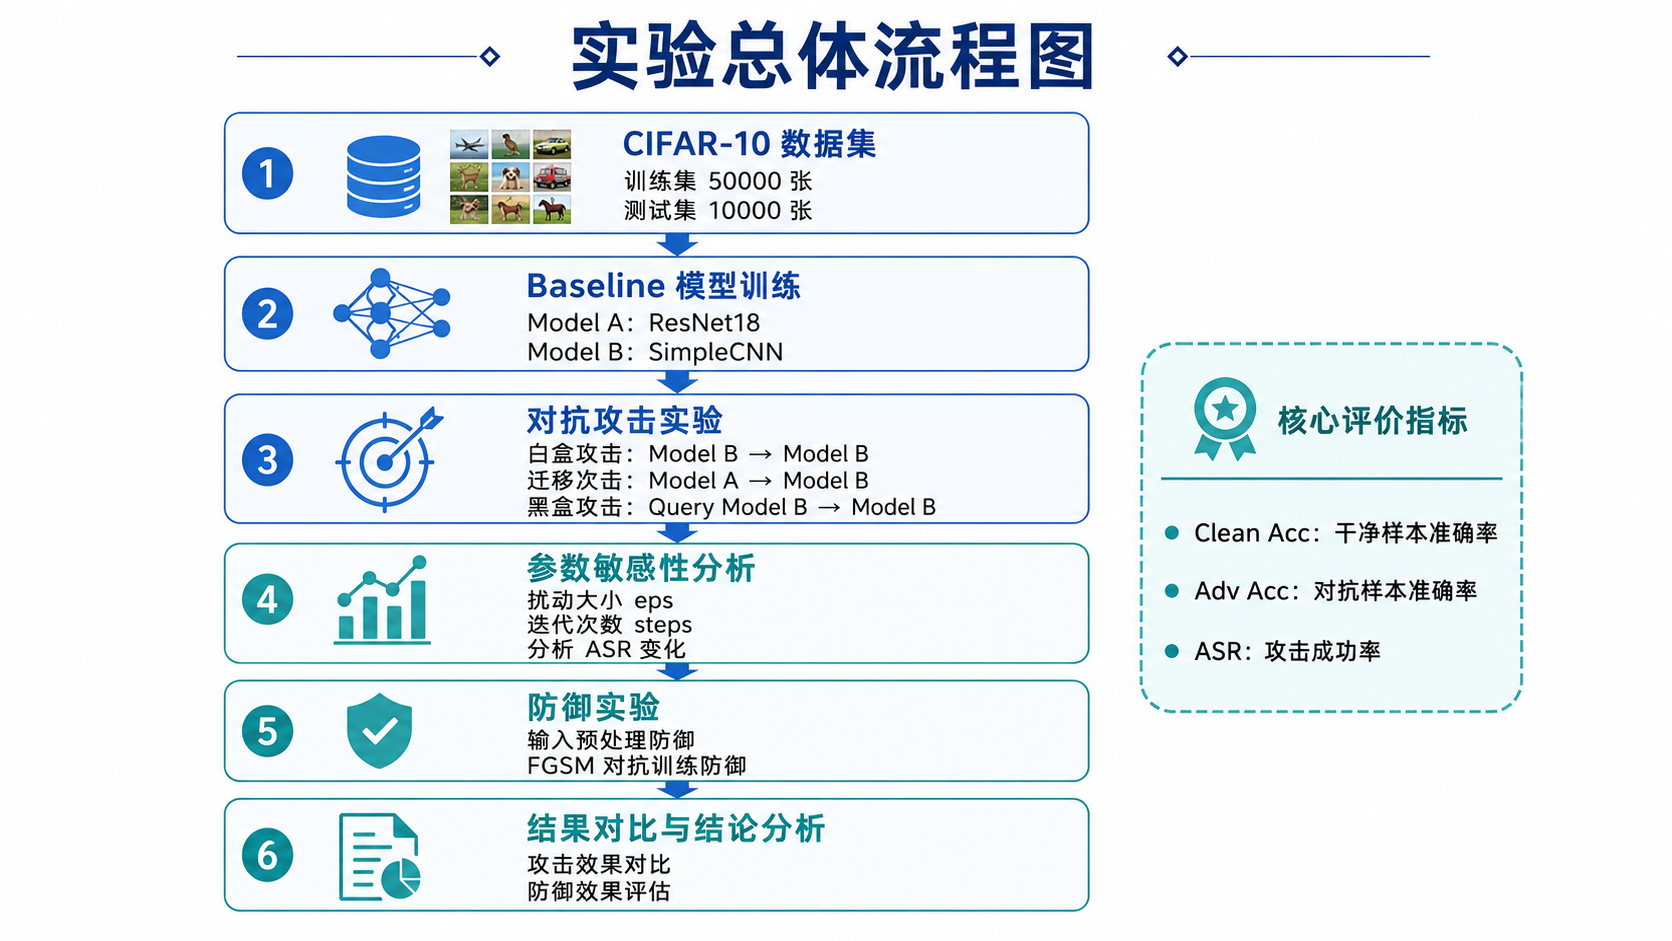
\includegraphics[width=0.90\textwidth]{figure/实验流程图.png}
    \caption{总体实验流程图}
    \label{fig:workflow}
\end{figure}

实验首先采用 CIFAR-10 数据集作为图像分类任务基础数据集。随后训练两个 baseline 模型，其中 Model A 采用 ResNet18 结构，Model B 采用 SimpleCNN 结构。接着分别进行白盒攻击、迁移攻击和黑盒攻击实验，并通过改变 eps 和 steps 分析攻击参数影响。最后设计输入预处理防御和对抗训练防御，并进一步使用 BPDA 自适应攻击、t-SNE 可视化和脆弱类别分析评价模型鲁棒性。

本项目的主要创新点包括：

\begin{enumerate}
    \item 在同一实验框架下同时比较白盒攻击、迁移攻击与查询型黑盒攻击，形成完整的攻击能力对照；
    \item 将输入预处理防御与对抗训练防御放在统一指标下评估，并进一步采用 BPDA 自适应攻击验证预处理防御的真实有效性；
    \item 结合 t-SNE 特征分布、扰动放大可视化和脆弱类别统计，从特征空间与样本层面对鲁棒性问题进行解释。
\end{enumerate}

\subsection{数据集与模型架构}

\subsubsection{数据集}

本实验采用 CIFAR-10 数据集。CIFAR-10 是图像分类任务中的经典数据集，包含 10 个类别的彩色图像，每张图像大小为 $32 \times 32$ 像素。数据集共包含 60000 张图像，其中训练集 50000 张，测试集 10000 张。10 个类别分别为 airplane、automobile、bird、cat、deer、dog、frog、horse、ship 和 truck。

在本实验中，训练集用于训练 baseline 分类模型，测试集用于评估模型在干净样本和对抗样本上的分类性能。

\begin{figure}[H]
    \centering
    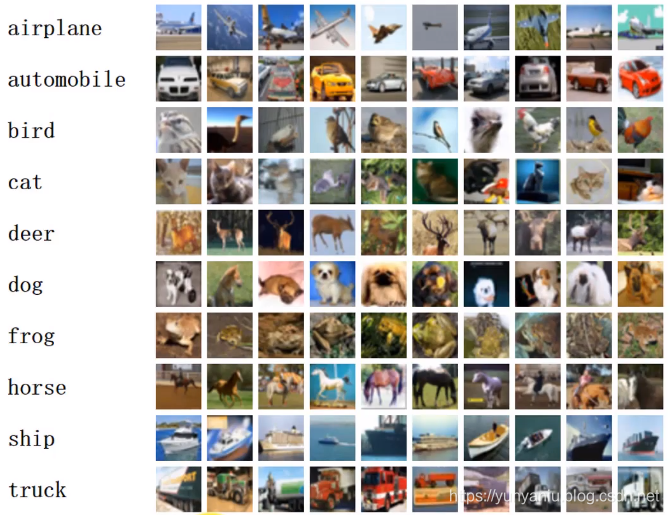
\includegraphics[width=0.90\textwidth]{figure/数据集介绍.png}
    \caption{CIFAR-10 数据集示意}
    \label{fig:dataset}
\end{figure}

\subsubsection{模型架构}

本实验训练两个 baseline 分类模型。Model A 采用 ResNet18 结构，主要作为迁移攻击中的源模型；Model B 采用 SimpleCNN 结构，作为主要被攻击模型，用于白盒攻击、黑盒攻击和迁移攻击评估。

其中，SimpleCNN 采用三段 ``卷积 + BatchNorm + ReLU + 最大池化'' 特征提取结构，并接两层全连接分类头；ResNet18 则将首层卷积调整为适配 $32 \times 32$ 输入的 $3 \times 3$、stride=1 结构，同时移除 ImageNet 场景中的首个最大池化层，以提升小分辨率图像上的特征保留能力。

\begin{table}[H]
    \centering
    \caption{Baseline 模型训练结果}
    \begin{tabular}{cccc}
        \toprule
        模型 & 网络结构 & 实验作用 & Clean Acc \\
        \midrule
        Model A & ResNet18 & 迁移攻击源模型 & 93.37\% \\
        Model B & SimpleCNN & 主要被攻击模型 & 91.62\% \\
        \bottomrule
    \end{tabular}
    \label{tab:baseline}
\end{table}

由于两个模型在干净测试集上均具有较高准确率，因此后续攻击实验中的准确率下降主要可以归因于对抗扰动的影响。

\subsection{攻击方法}

\subsubsection{攻击场景划分}

根据攻击者掌握目标模型信息的不同，本实验将攻击场景划分为白盒攻击、黑盒攻击和迁移攻击三类。

\begin{table}[H]
    \centering
    \caption{攻击场景划分}
    \resizebox{\textwidth}{!}{
    \begin{tabular}{p{2.2cm}p{4.4cm}p{3.6cm}p{4.5cm}}
        \toprule
        攻击场景 & 攻击者掌握的信息 & 攻击路径 & 本实验使用方法 \\
        \midrule
        白盒攻击 & 知道模型结构、参数和梯度 & Model B $\rightarrow$ Model B & FGSM、PGD、DeepFool \\
        黑盒攻击 & 不知道模型结构和梯度，只能查询输出 & Query Model B $\rightarrow$ Model B & SPSA \\
        迁移攻击 & 知道源模型，不知道目标模型梯度 & Model A $\rightarrow$ Model B & FGSM、PGD、MI-FGSM、DeepFool \\
        \bottomrule
    \end{tabular}
    }
    \label{tab:attack_scenarios}
\end{table}

\subsubsection{FGSM 攻击}

FGSM，全称 Fast Gradient Sign Method，是一种单步白盒攻击方法。其核心思想是计算损失函数对输入图像的梯度方向，并沿梯度符号方向添加扰动，使模型损失增大，从而导致误分类。

\begin{equation}
    x_{\mathrm{adv}} = x + \epsilon \cdot \mathrm{sign}(\nabla_x J(\theta, x, y))
\end{equation}

其中，$x$ 表示原始图像，$x_{\mathrm{adv}}$ 表示对抗样本，$\epsilon$ 表示扰动上限，$J(\theta,x,y)$ 表示模型损失函数。
\begin{figure}[H]
    \centering
    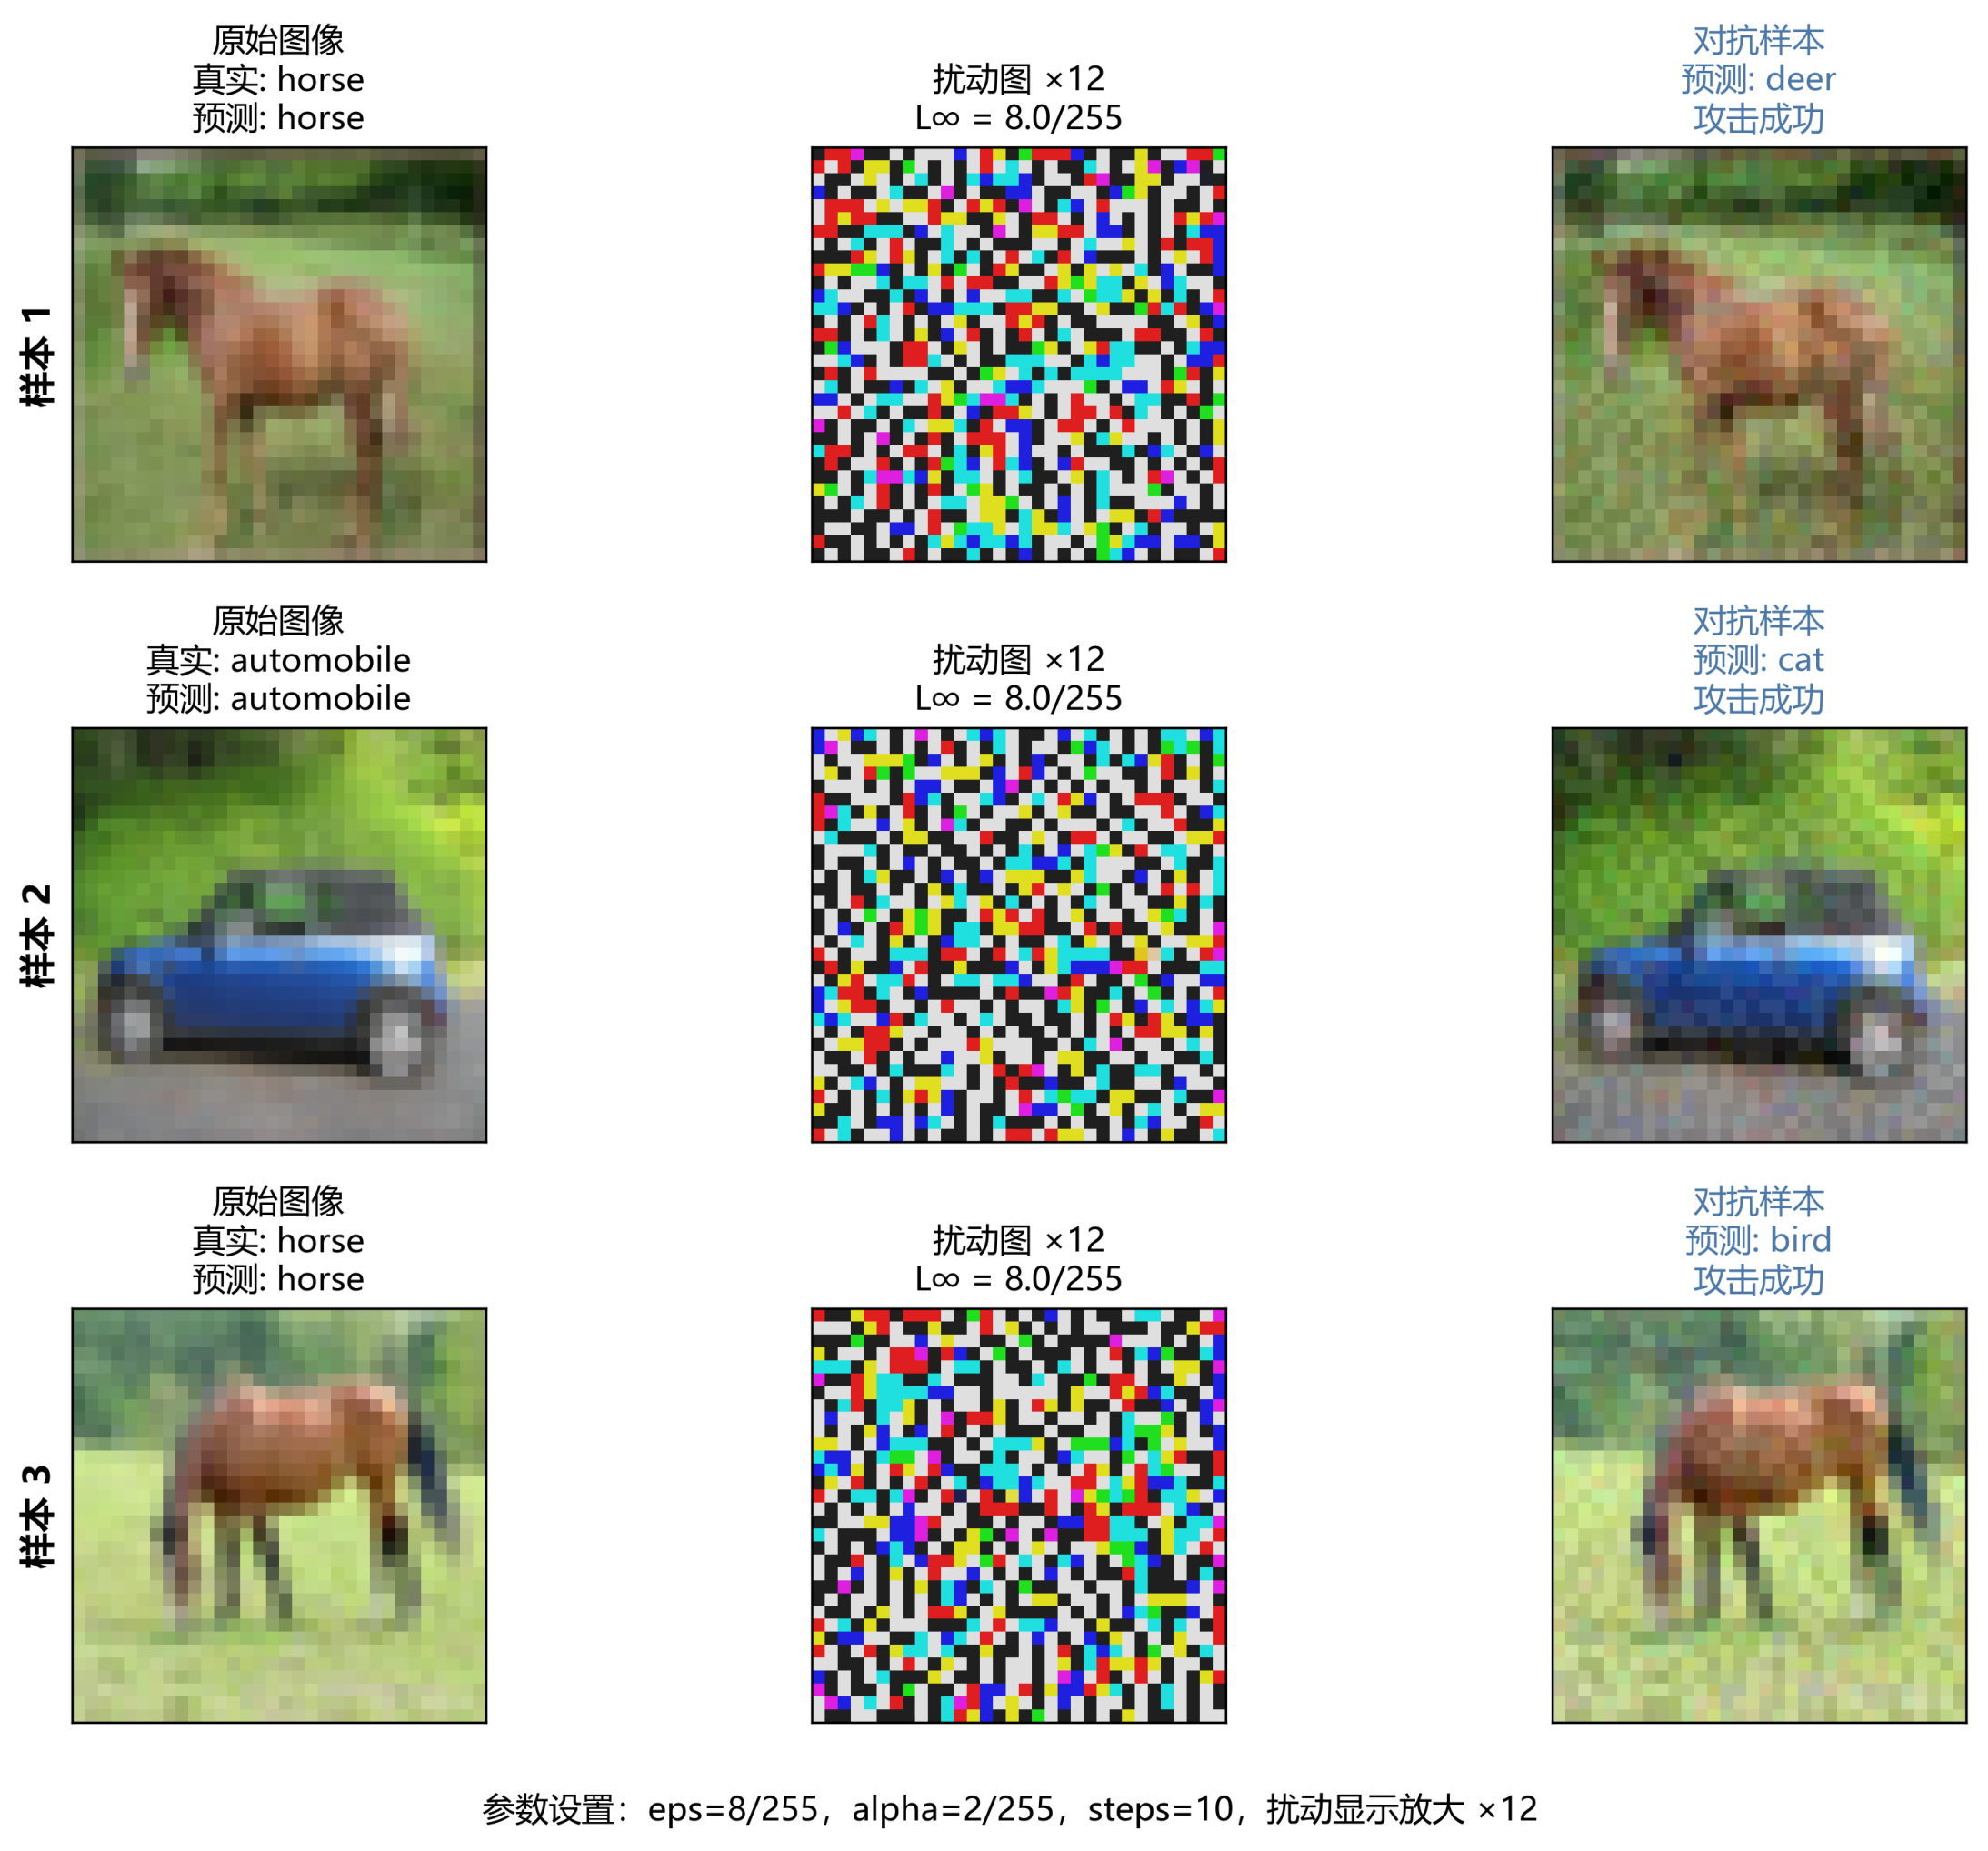
\includegraphics[width=0.90\textwidth]{figure/fgsm.png}
    \caption{FGSM攻击}
    \label{fig:FGSM}
\end{figure}

\subsubsection{PGD 攻击}

PGD，全称 Projected Gradient Descent，可以看作 FGSM 的多步迭代增强版本。PGD 每一步沿梯度方向更新对抗样本，并将扰动投影回 $\epsilon$ 邻域内。

\begin{equation}
    x_{t+1} = \Pi_{B_{\epsilon}(x)} 
    \left[
    x_t + \alpha \cdot \mathrm{sign}(\nabla_x J(\theta, x_t, y))
    \right]
\end{equation}

其中，$\alpha$ 表示每一步更新步长，$\Pi_{B_{\epsilon}(x)}$ 表示投影操作，用于保证扰动不超过允许范围。

\begin{figure}[H]
    \centering
    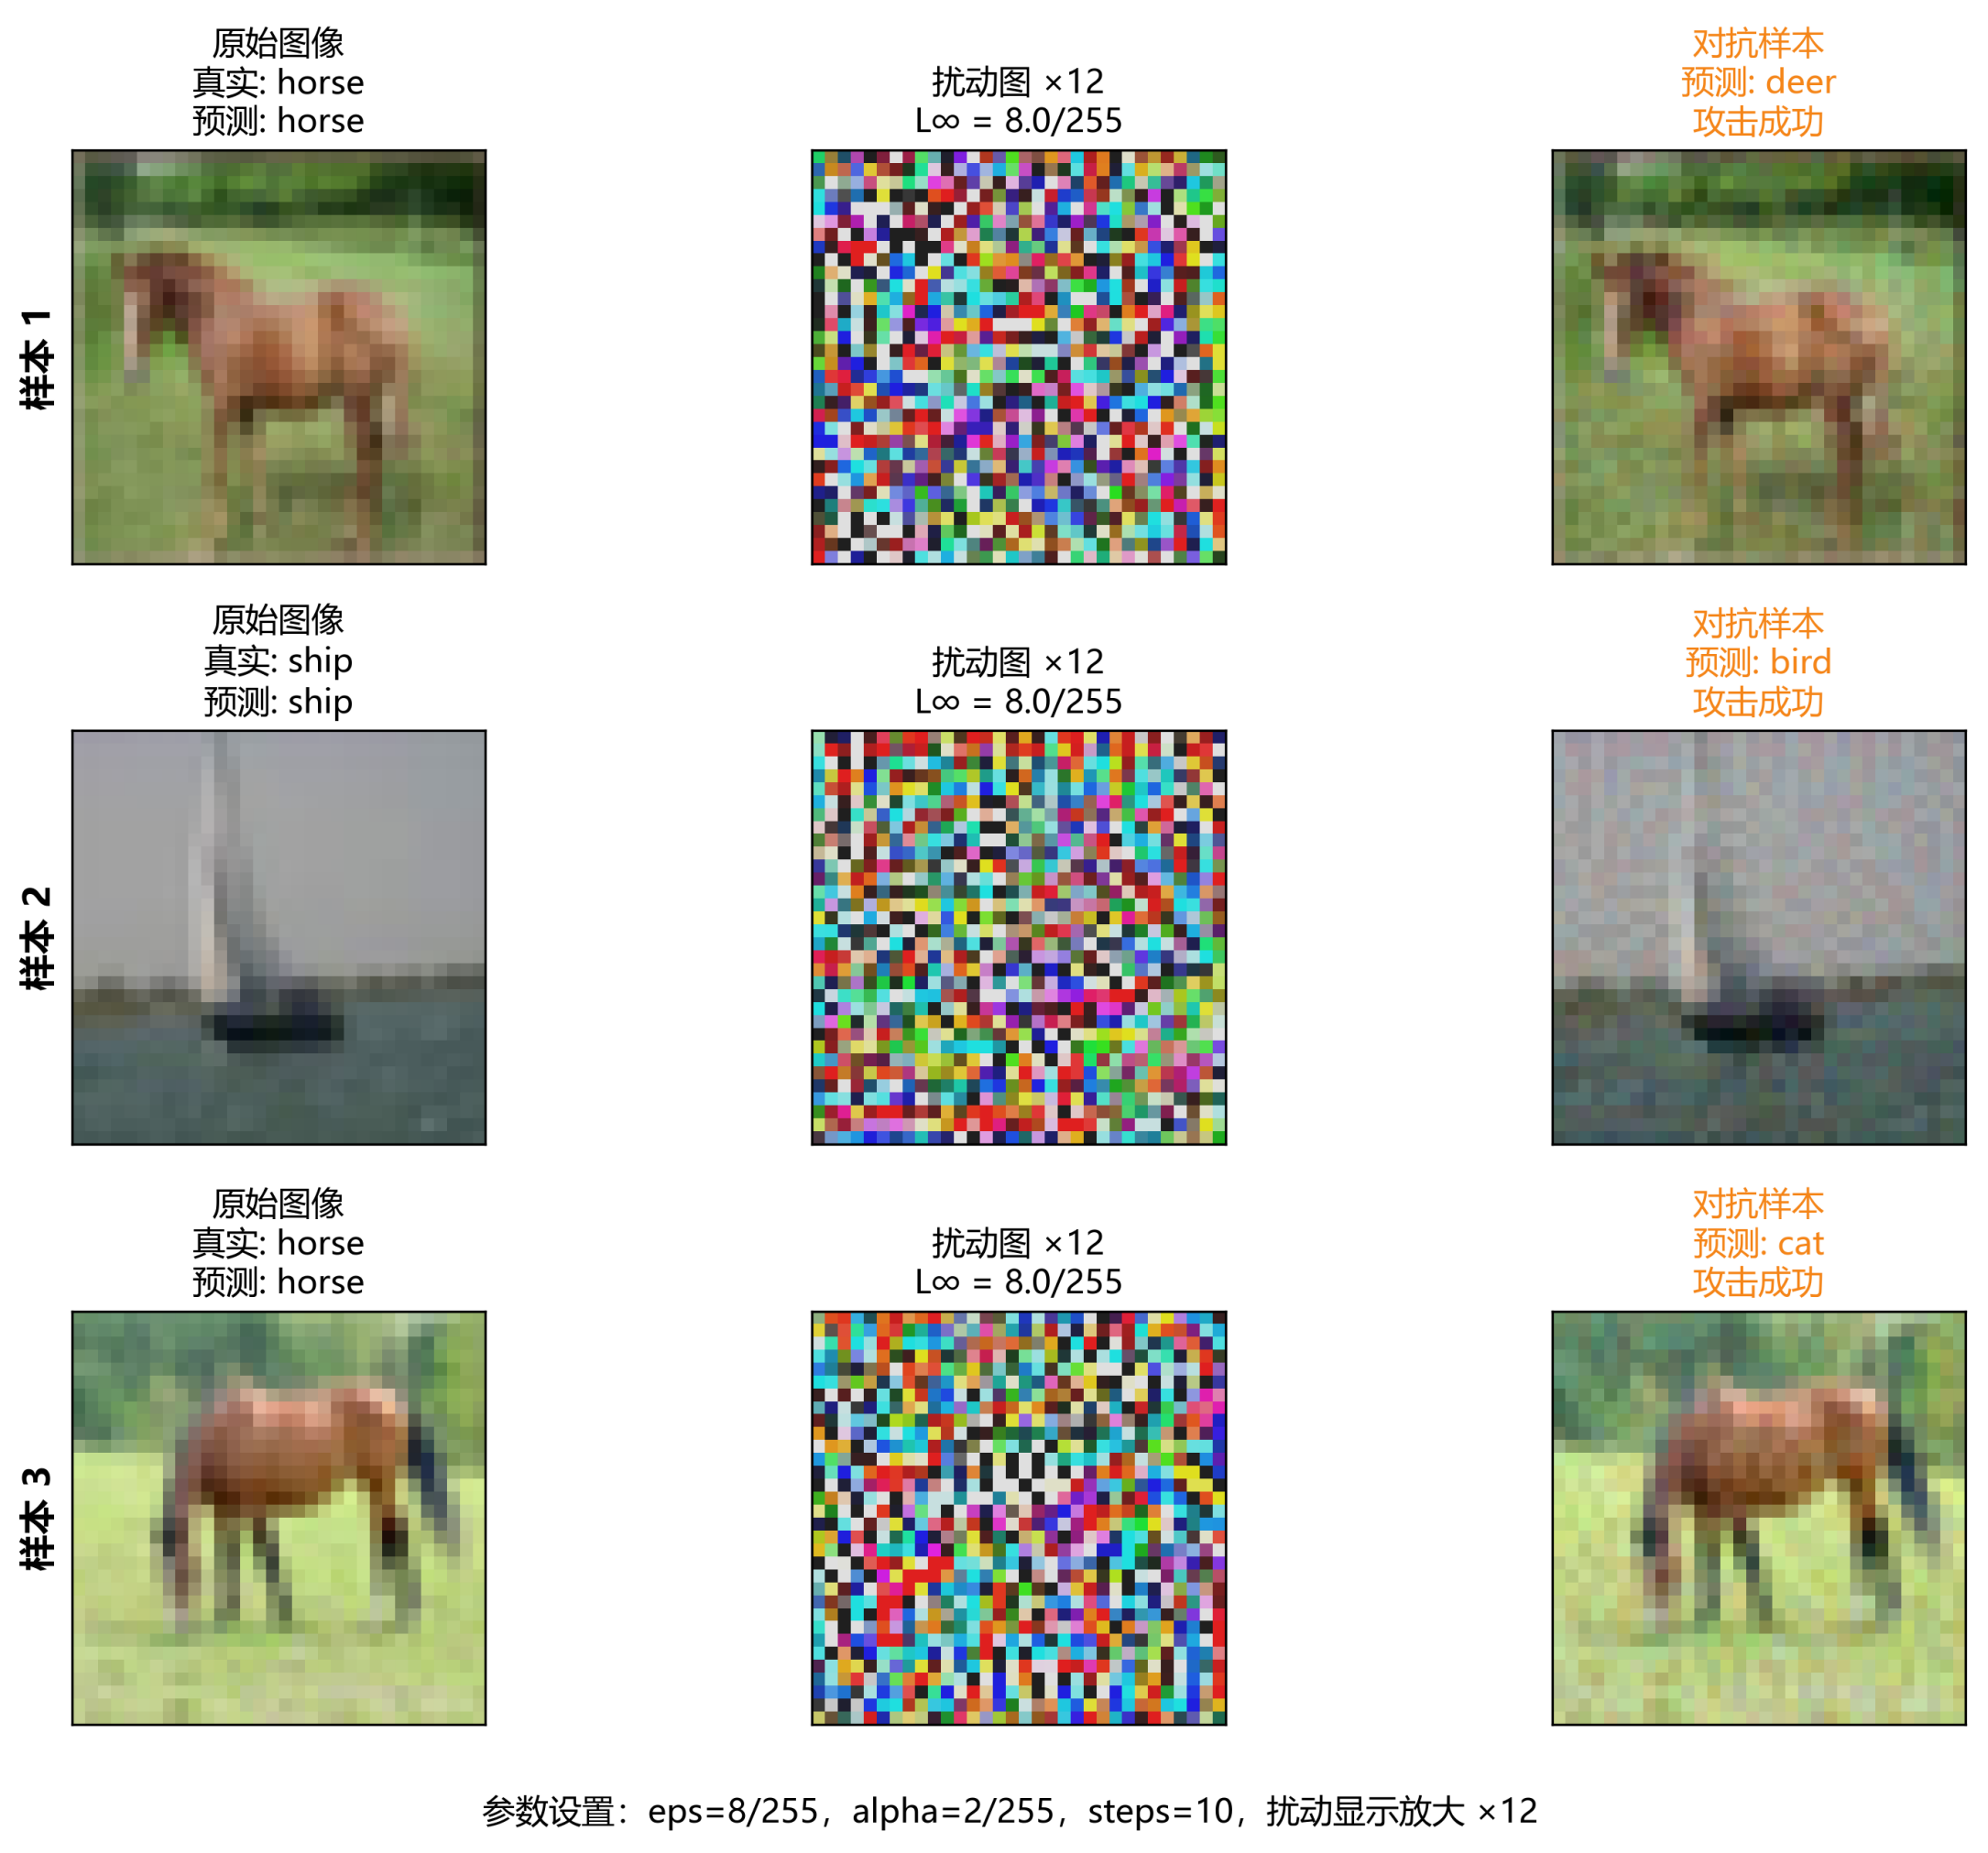
\includegraphics[width=0.90\textwidth]{figure/pgd.png}
    \caption{PGD攻击}
    \label{fig:PGD}
\end{figure}


\subsubsection{DeepFool 攻击}

DeepFool 是一种基于分类边界的迭代攻击方法，其目标是寻找使样本越过决策边界所需的近似最小扰动。其优化目标可以表示为：

\begin{equation}
    \min \|r\|_2, \quad 
    \mathrm{s.t.}\ \hat{k}(x+r) \neq \hat{k}(x)
\end{equation}

其中，$r$ 表示扰动，$\hat{k}(x)$ 表示模型对输入 $x$ 的预测类别。

\begin{figure}[H]
    \centering
    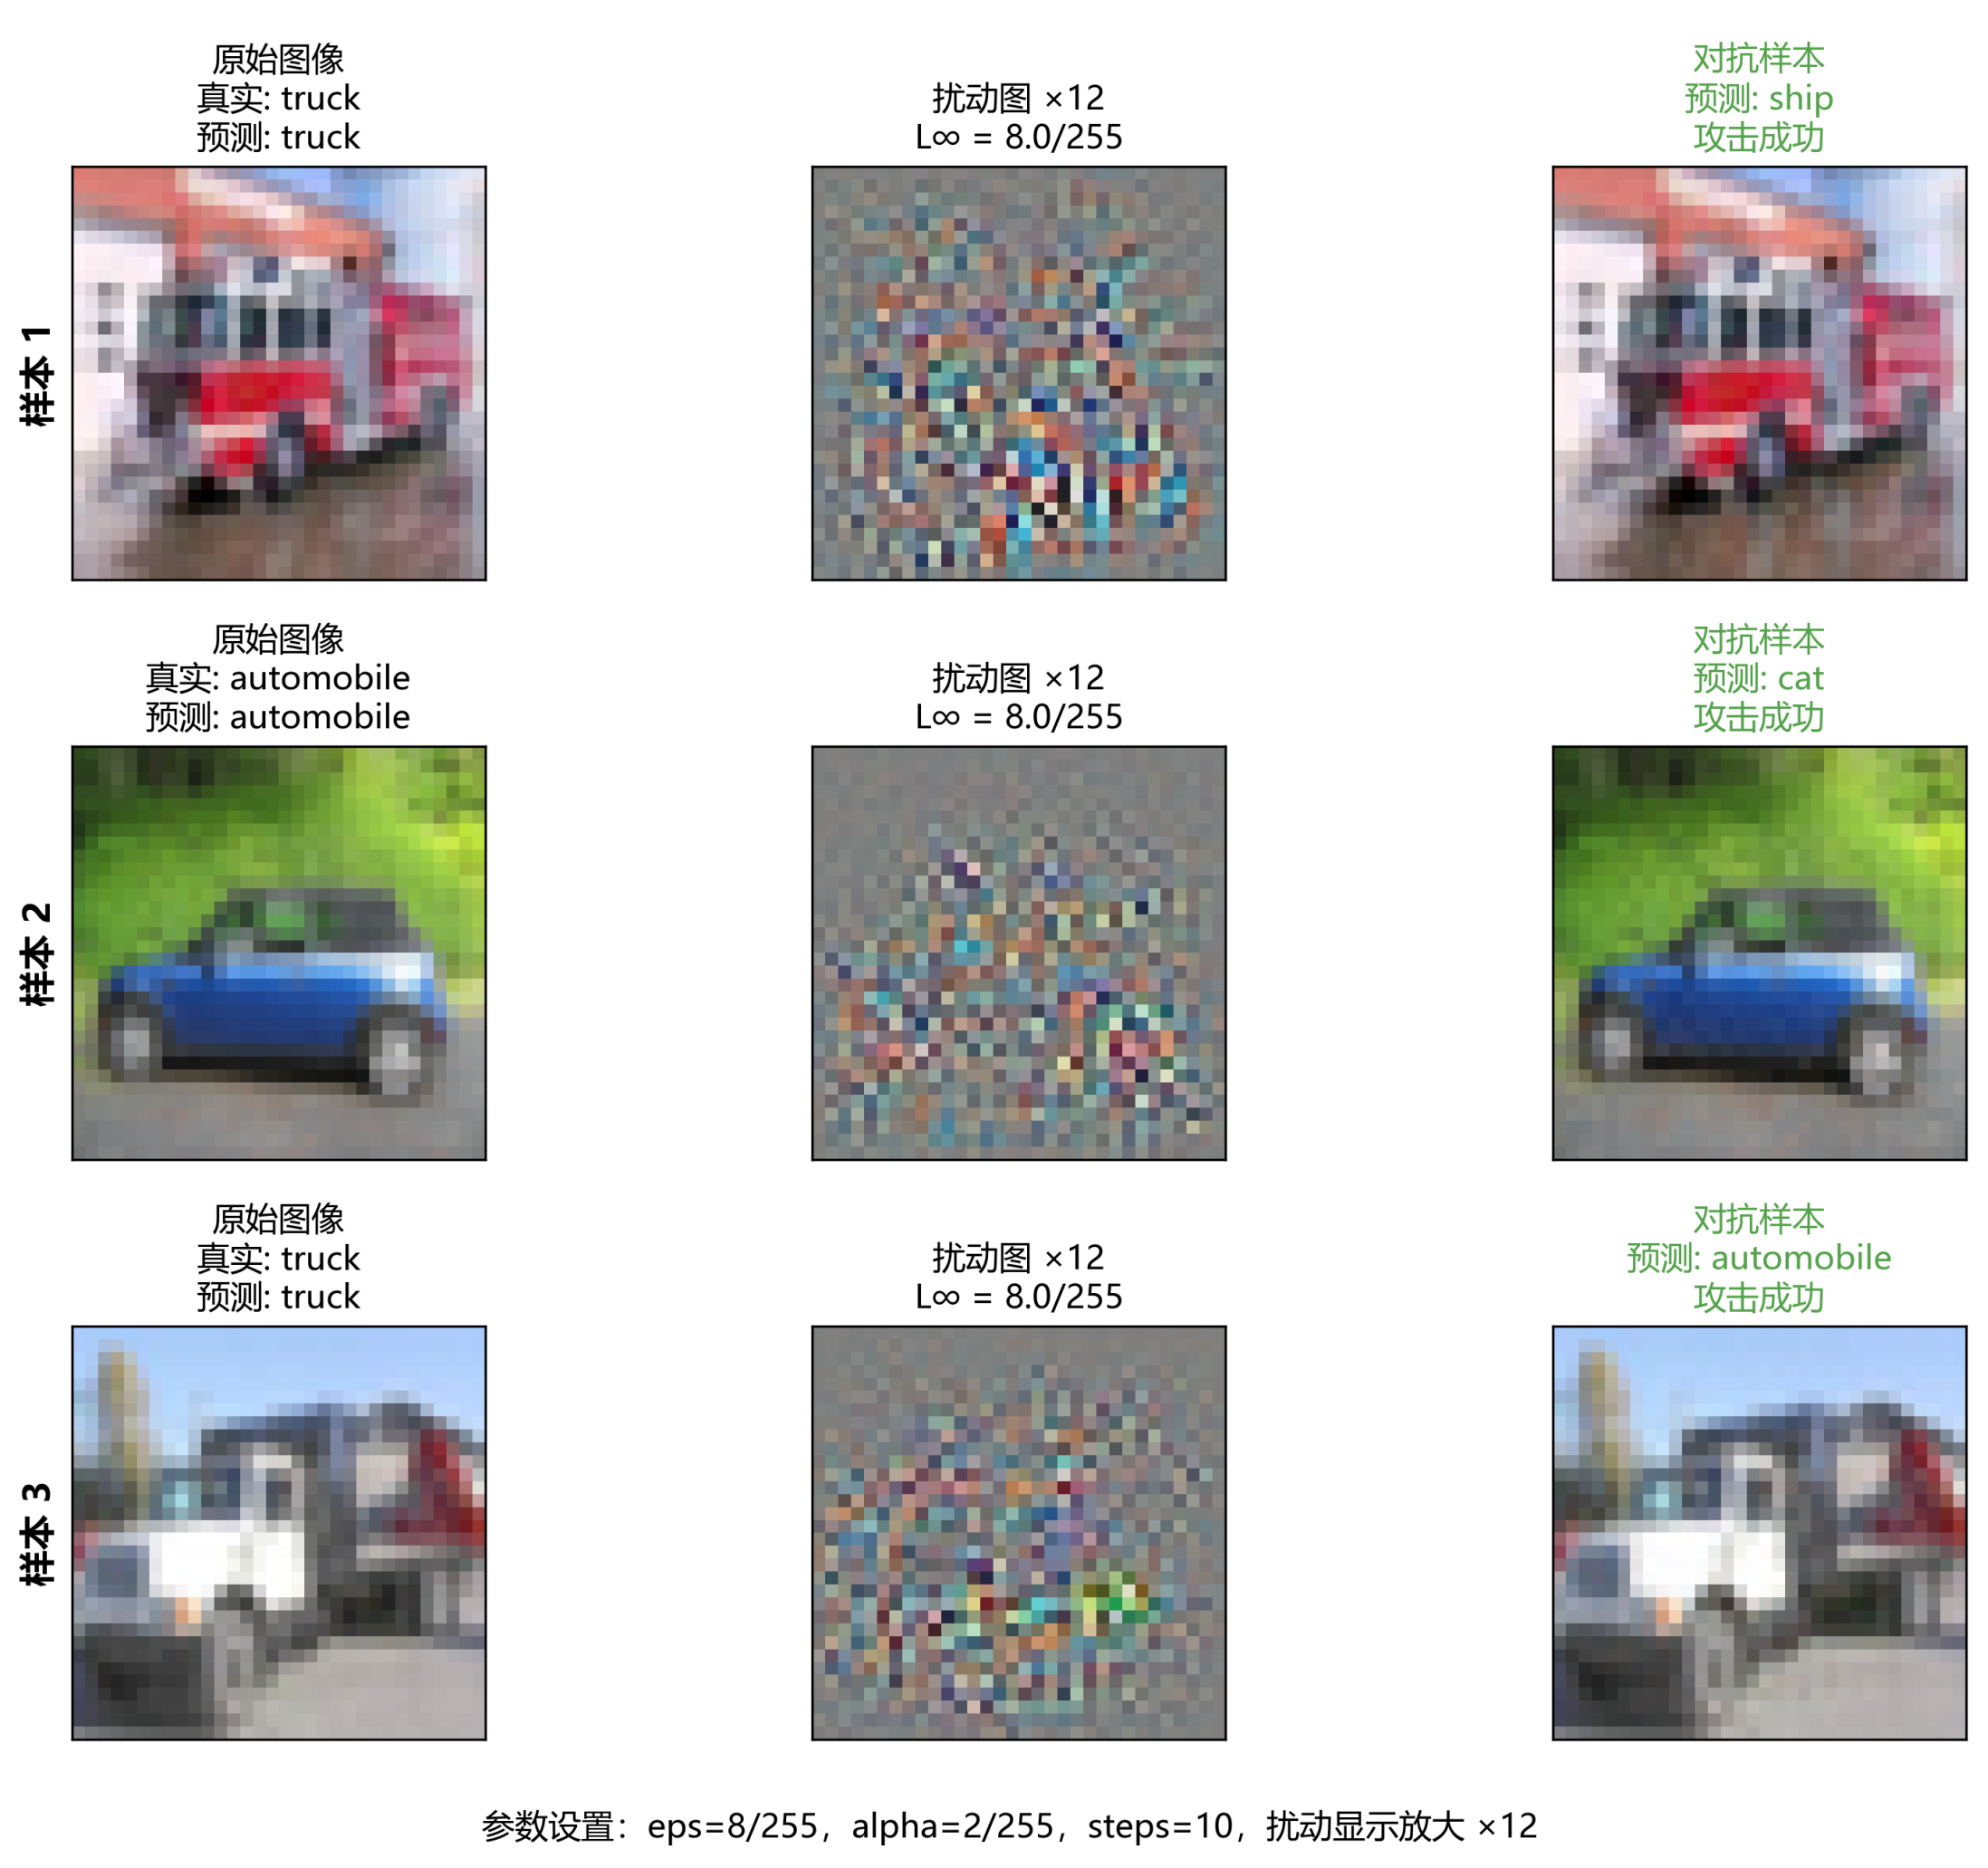
\includegraphics[width=0.90\textwidth]{figure/deepfool.png}
    \caption{DeepFool攻击}
    \label{fig:DeepFool}
\end{figure}

\subsubsection{三种典型攻击的可视化对比}

为了更直观地比较 FGSM、PGD 和 DeepFool 三种攻击方式，本文选取若干 CIFAR-10 测试样本，将原始图像与三种攻击生成的对抗样本进行并列展示，如图~\ref{fig:attack_compare} 所示。

从图中可以看出，三种攻击生成的对抗样本在视觉上与原始图像差别较小，但都已经引入了能够误导模型预测的扰动。其中，FGSM 属于单步攻击，扰动相对直接；PGD 属于多步迭代攻击，通常能够产生更强的攻击效果；DeepFool 则倾向于寻找使样本跨越分类边界的最小扰动，因此其视觉变化往往更加细微。

\begin{figure}[H]
    \centering
    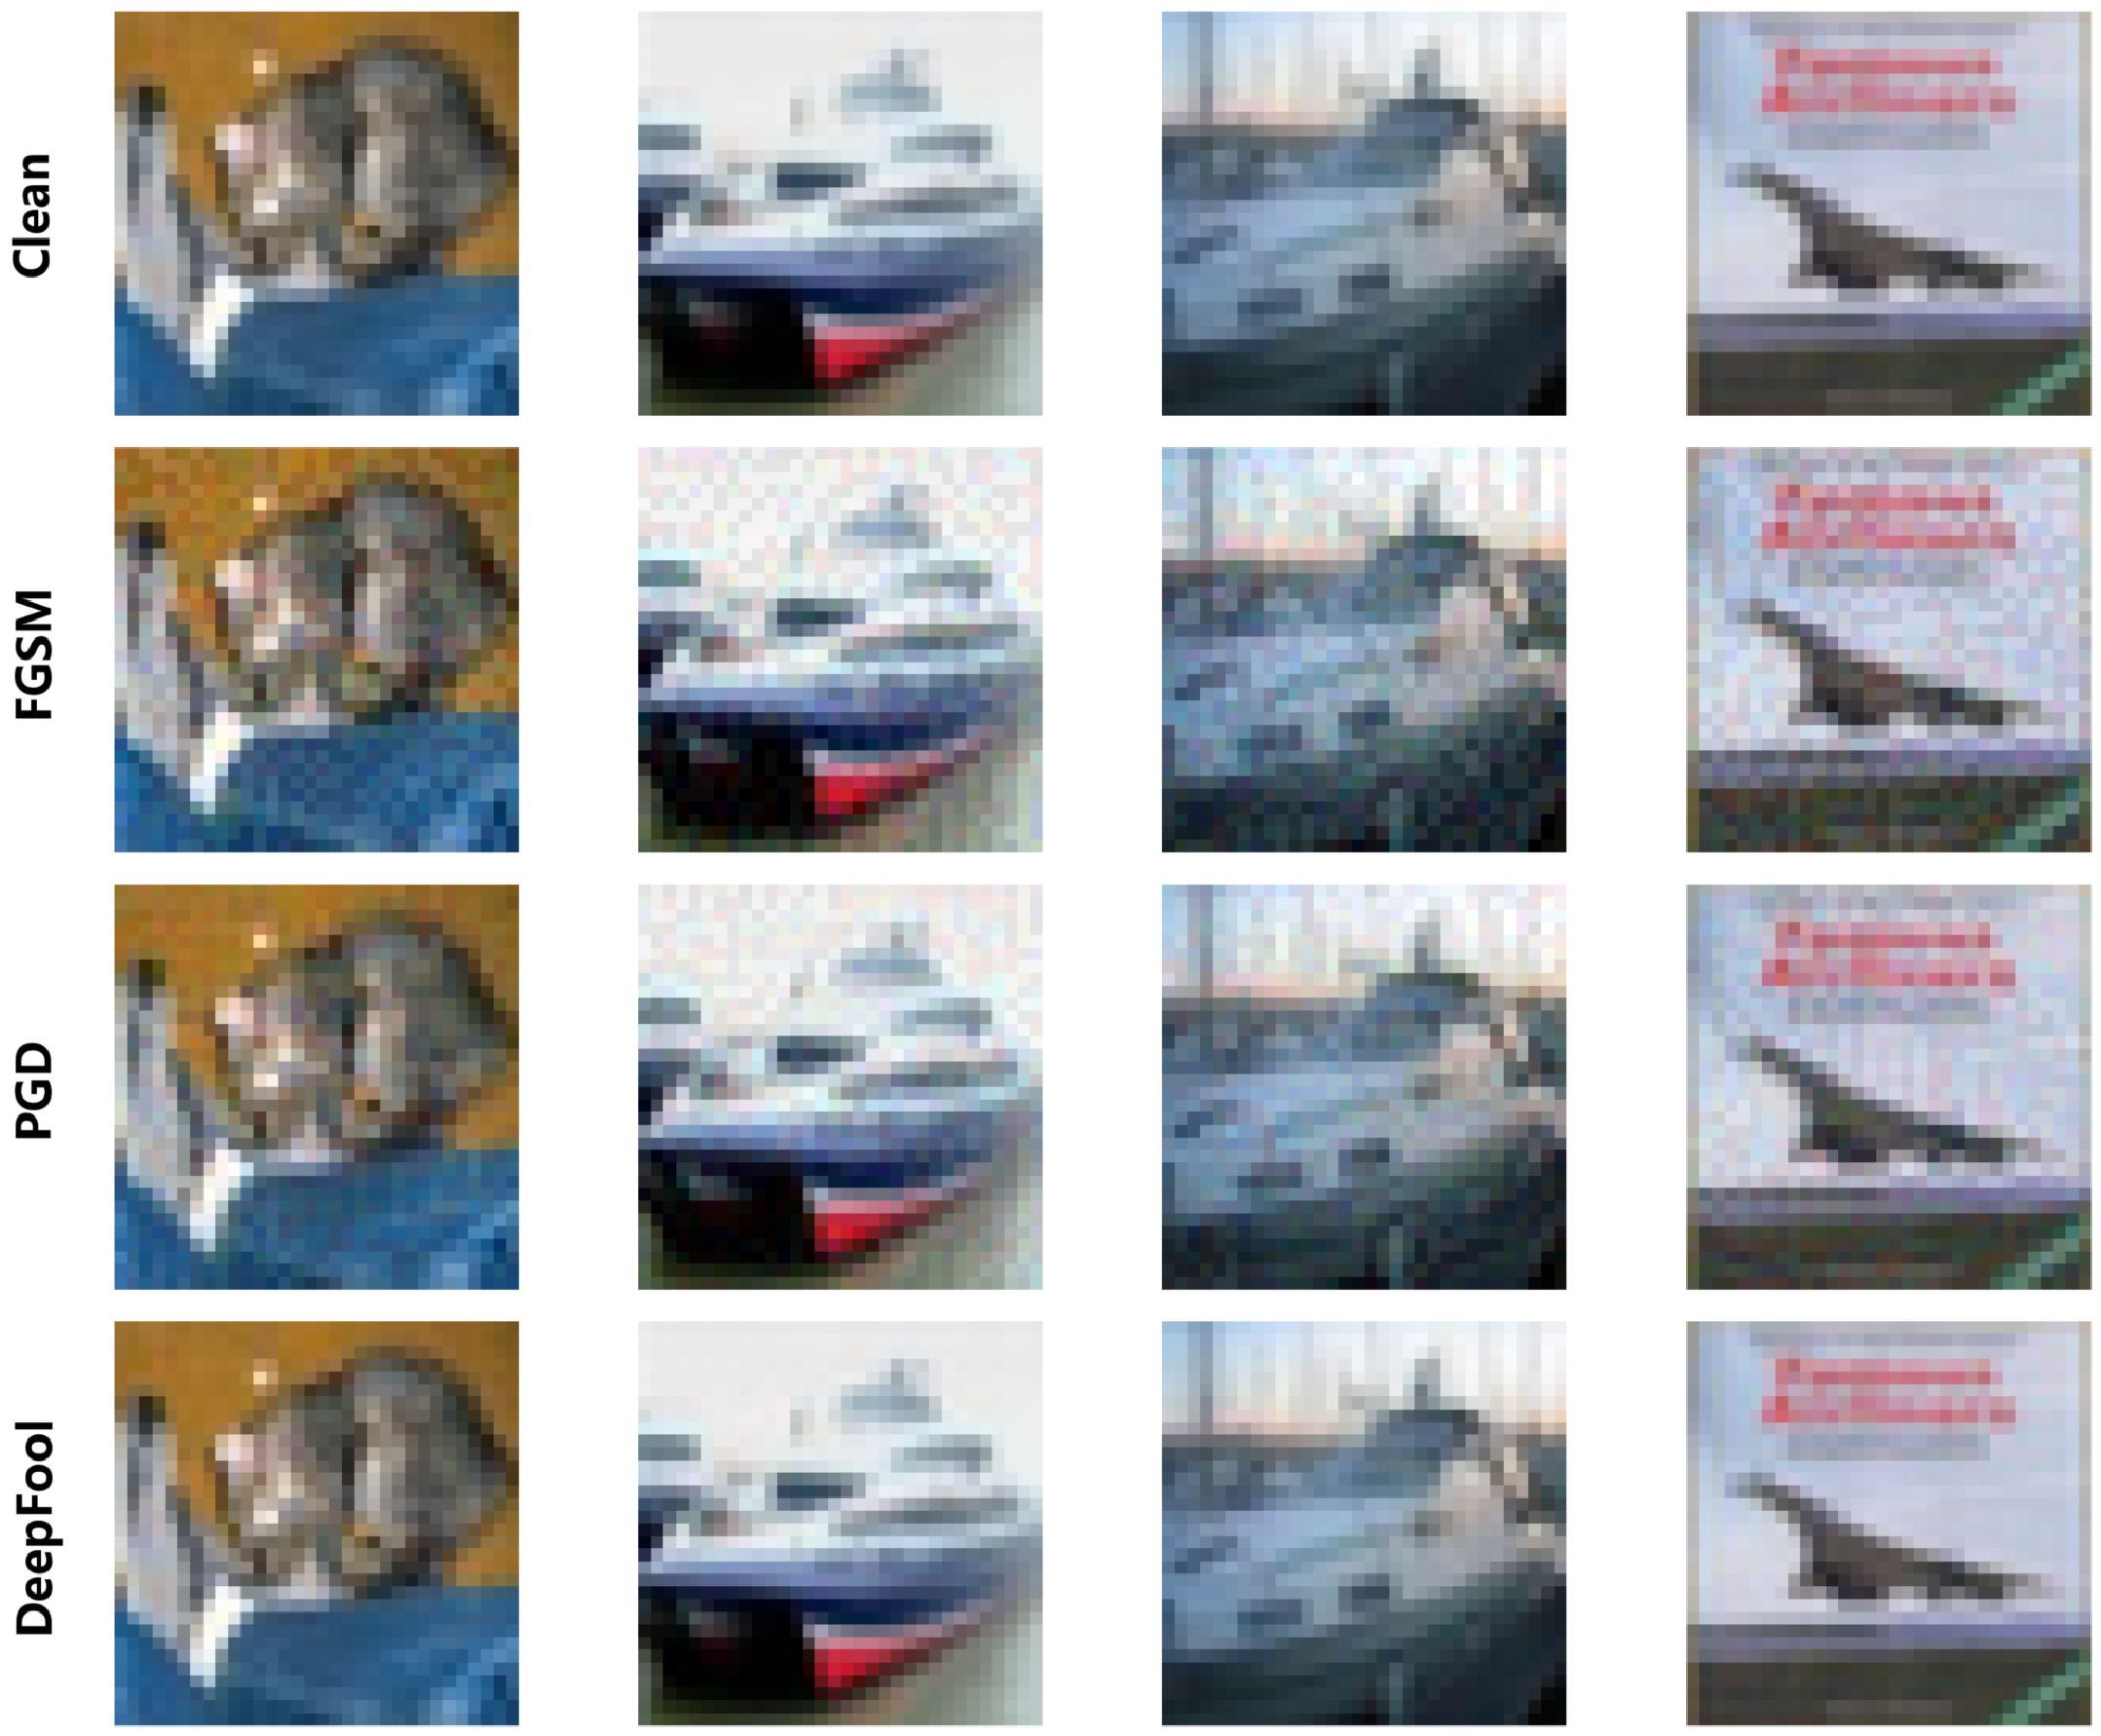
\includegraphics[width=0.88\textwidth]{figure/攻击.png}
    \caption{FGSM、PGD 和 DeepFool 三种攻击的可视化对比}
    \label{fig:attack_compare}
\end{figure}

\subsubsection{MI-FGSM 攻击}

MI-FGSM 是 Momentum Iterative FGSM 的缩写。它在迭代梯度攻击中加入动量项，使攻击方向更加稳定，从而增强对抗样本的迁移能力。其更新过程为：

\begin{equation}
    g_{t+1} = \mu g_t +
    \frac{\nabla_x J(\theta, x_t, y)}
    {\|\nabla_x J(\theta, x_t, y)\|_1}
\end{equation}

\begin{equation}
    x_{t+1} = x_t + \alpha \cdot \mathrm{sign}(g_{t+1})
\end{equation}

\subsubsection{SPSA 攻击}

SPSA，全称 Simultaneous Perturbation Stochastic Approximation，是一种黑盒随机梯度估计方法。它不需要直接获取模型结构和梯度，而是通过多次查询模型输出结果估计输入方向上的梯度变化。由于 SPSA 只依赖模型输出，因此更接近实际黑盒攻击场景，但查询成本较高。

\subsection{防御思路}

本实验采用两类防御思路。第一类是输入预处理防御，包括 JPEG 压缩与位深压缩，其目标是在推理阶段削弱高频扰动；第二类是对抗训练防御，包括 FGSM 与 PGD 对抗训练，其目标是在训练阶段显式引入对抗样本，从而提高模型在强攻击下的鲁棒性。为避免简单预处理产生梯度遮蔽假象，本文进一步采用 BPDA 自适应攻击评估其真实安全性。

% =========================================================
\section{实验}
% =========================================================

\subsection{实验设置}

实验默认设置为扰动大小 $\epsilon=8/255$、步长 $\alpha=2/255$、迭代次数 steps=10。白盒攻击在 Model B 上直接生成并评估对抗样本；迁移攻击在 Model A 上生成对抗样本并迁移到 Model B；黑盒攻击使用 SPSA 通过查询方式估计梯度。对抗训练实验分别比较 FGSM 与 PGD 训练策略，输入预处理实验则统一在 JPEG 质量 75 和位深 5 bit 的设定下进行。

\subsection{评价指标}

本实验主要使用以下评价指标：

\begin{itemize}
    \item Clean Acc：模型在干净样本上的准确率；
    \item Adv Acc：模型在对抗样本上的准确率；
    \item ASR：攻击成功率，即原本分类正确但攻击后分类错误的样本比例。
\end{itemize}

\subsection{攻击实验结果}

\begin{table}[H]
    \centering
    \caption{攻击实验结果}
    \resizebox{\textwidth}{!}{
    \begin{tabular}{ccccc}
        \toprule
        攻击类型 & 攻击方法 & 攻击路径 & Adv Acc & ASR \\
        \midrule
        白盒攻击 & FGSM & Model B $\rightarrow$ Model B & 11.97\% & 86.96\% \\
        白盒攻击 & PGD & Model B $\rightarrow$ Model B & 0.26\% & 99.72\% \\
        白盒攻击 & DeepFool & Model B $\rightarrow$ Model B & 17.59\% & 86.53\% \\
        迁移攻击 & FGSM & Model A $\rightarrow$ Model B & 38.96\% & 57.73\% \\
        迁移攻击 & PGD & Model A $\rightarrow$ Model B & 20.26\% & 77.88\% \\
        迁移攻击 & MI-FGSM & Model A $\rightarrow$ Model B & 12.78\% & 86.06\% \\
        迁移攻击 & DeepFool & Model A $\rightarrow$ Model B & 89.17\% & 2.87\% \\
        黑盒攻击 & SPSA & Query Model B $\rightarrow$ Model B & 41.90\% & 54.31\% \\
        \bottomrule
    \end{tabular}
    }
    \label{tab:attack_results}
\end{table}

由表~\ref{tab:attack_results} 可见，白盒 PGD 攻击最强，使 Model B 的 Adv Acc 降低到 0.26\%，ASR 达到 99.72\%。在迁移攻击中，MI-FGSM 的 ASR 达到 86.06\%，说明动量机制能够显著提升跨模型攻击能力。相比之下，Transfer DeepFool 的 ASR 仅为 2.87\%，说明 DeepFool 生成的最小扰动高度依赖源模型决策边界，迁移能力较弱。

\subsection{扰动大小 eps 对攻击效果的影响}

本实验固定 steps=10，$\alpha=2/255$，改变扰动大小 eps，测试不同攻击方法的 Adv Acc 和 ASR。

\begin{table}[H]
    \centering
    \caption{扰动大小 eps 对攻击效果的影响}
    \resizebox{\textwidth}{!}{
    \begin{tabular}{cccccccc}
        \toprule
        攻击类型 & 攻击方法 & eps=2/255 & eps=4/255 & eps=8/255 & eps=12/255 & eps=16/255 \\
        \midrule
        白盒攻击 & FGSM & 31.71 / 65.36 & 15.92 / 82.62 & 11.97 / 86.96 & 11.16 / 87.93 & 10.61 / 88.61 \\
        白盒攻击 & PGD & 14.95 / 83.67 & 1.67 / 98.18 & 0.23 / 99.75 & 0.07 / 99.92 & 0.02 / 99.98 \\
        白盒攻击 & DeepFool & 49.89 / 51.08 & 27.46 / 75.67 & 17.47 / 86.64 & 15.74 / 88.53 & 15.21 / 89.13 \\
        迁移攻击 & FGSM & 74.49 / 18.66 & 58.32 / 36.37 & 38.96 / 57.73 & 28.67 / 69.35 & 21.15 / 77.59 \\
        迁移攻击 & PGD & 75.10 / 17.99 & 51.40 / 43.88 & 20.94 / 77.14 & 10.31 / 88.74 & 6.91 / 92.46 \\
        迁移攻击 & MI-FGSM & 70.96 / 22.56 & 42.53 / 53.54 & 12.78 / 86.06 & 4.28 / 95.34 & 2.25 / 97.55 \\
        \bottomrule
    \end{tabular}
    }
    \label{tab:eps_sensitivity}
\end{table}

表~\ref{tab:eps_sensitivity} 中单元格格式为 ``Adv Acc / ASR''，单位均为百分比。可以看出，随着扰动大小 eps 增大，攻击成功率整体上升，对抗样本准确率整体下降。白盒攻击中 PGD 最强，在 eps=8/255 时 ASR 已达到 99.75\%；迁移攻击中 MI-FGSM 对 eps 增大最敏感，ASR 从 22.56\% 提升到 97.55\%。

\begin{figure}[H]
    \centering

    \begin{subfigure}[b]{0.48\textwidth}
        \centering
        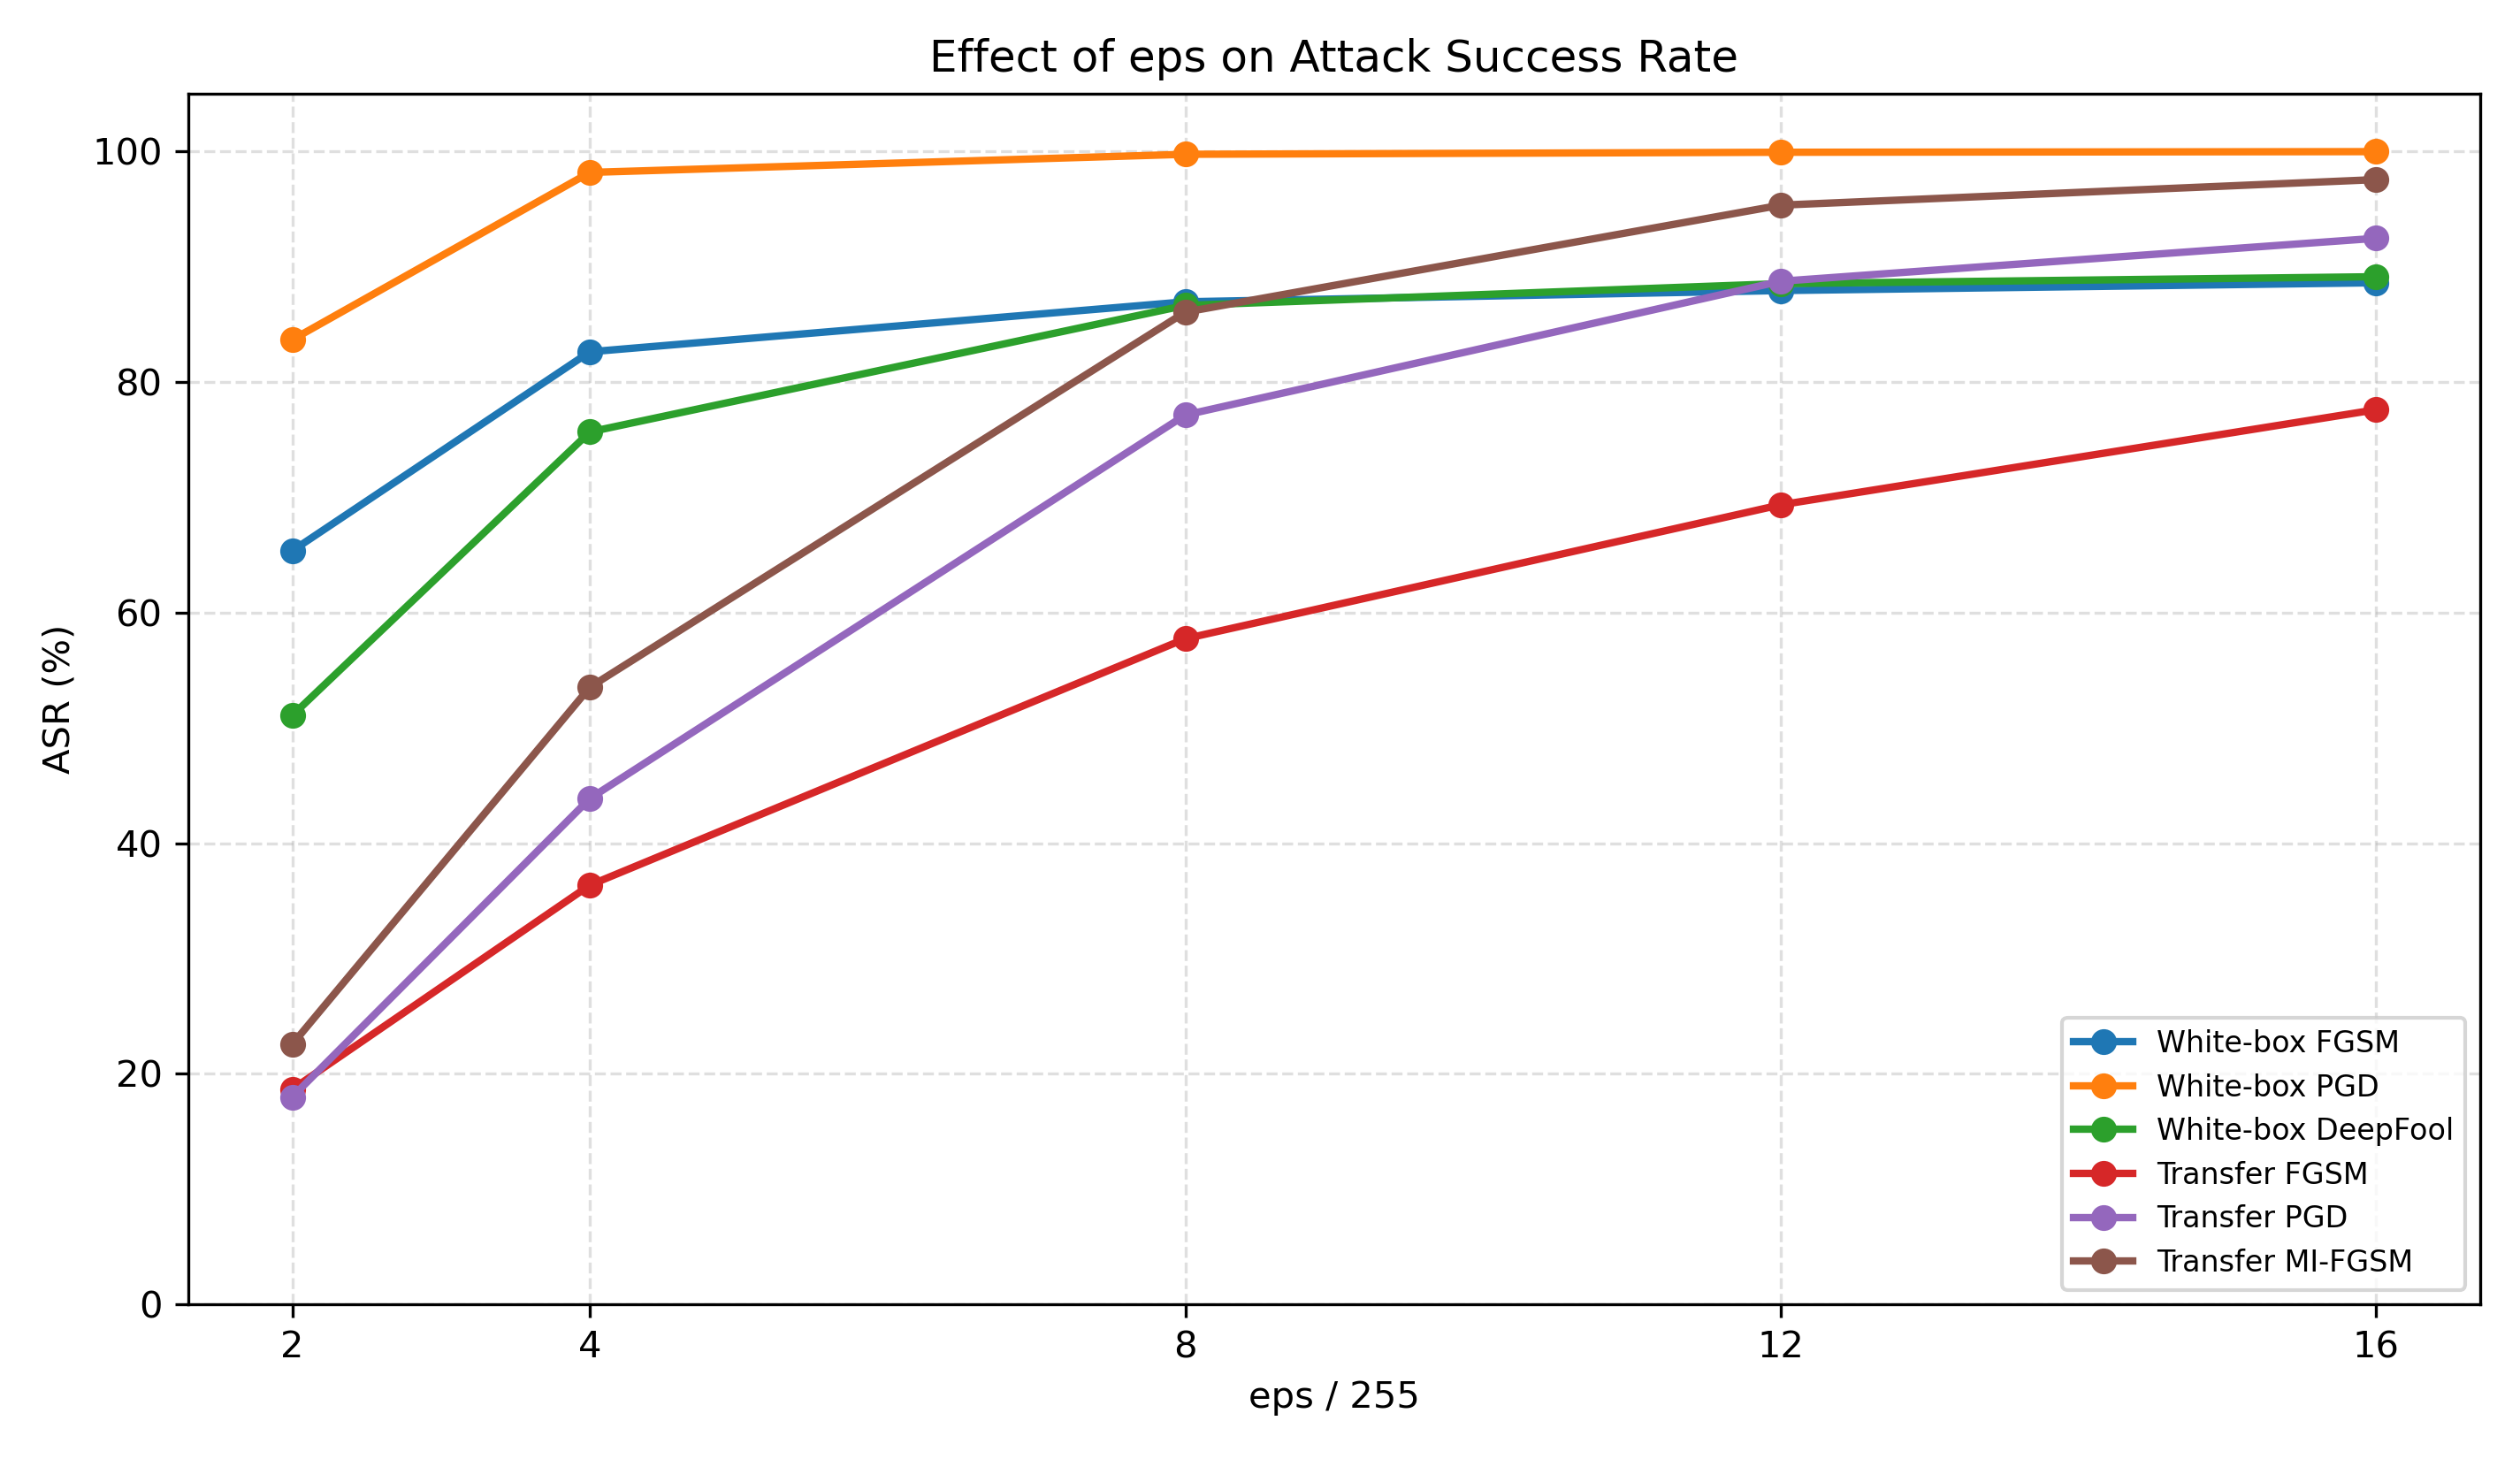
\includegraphics[width=\textwidth]{figure/eps1.png}
        \caption{eps 对攻击成功率 ASR 的影响}
        \label{fig:eps_asr}
    \end{subfigure}
    \hfill
    \begin{subfigure}[b]{0.48\textwidth}
        \centering
        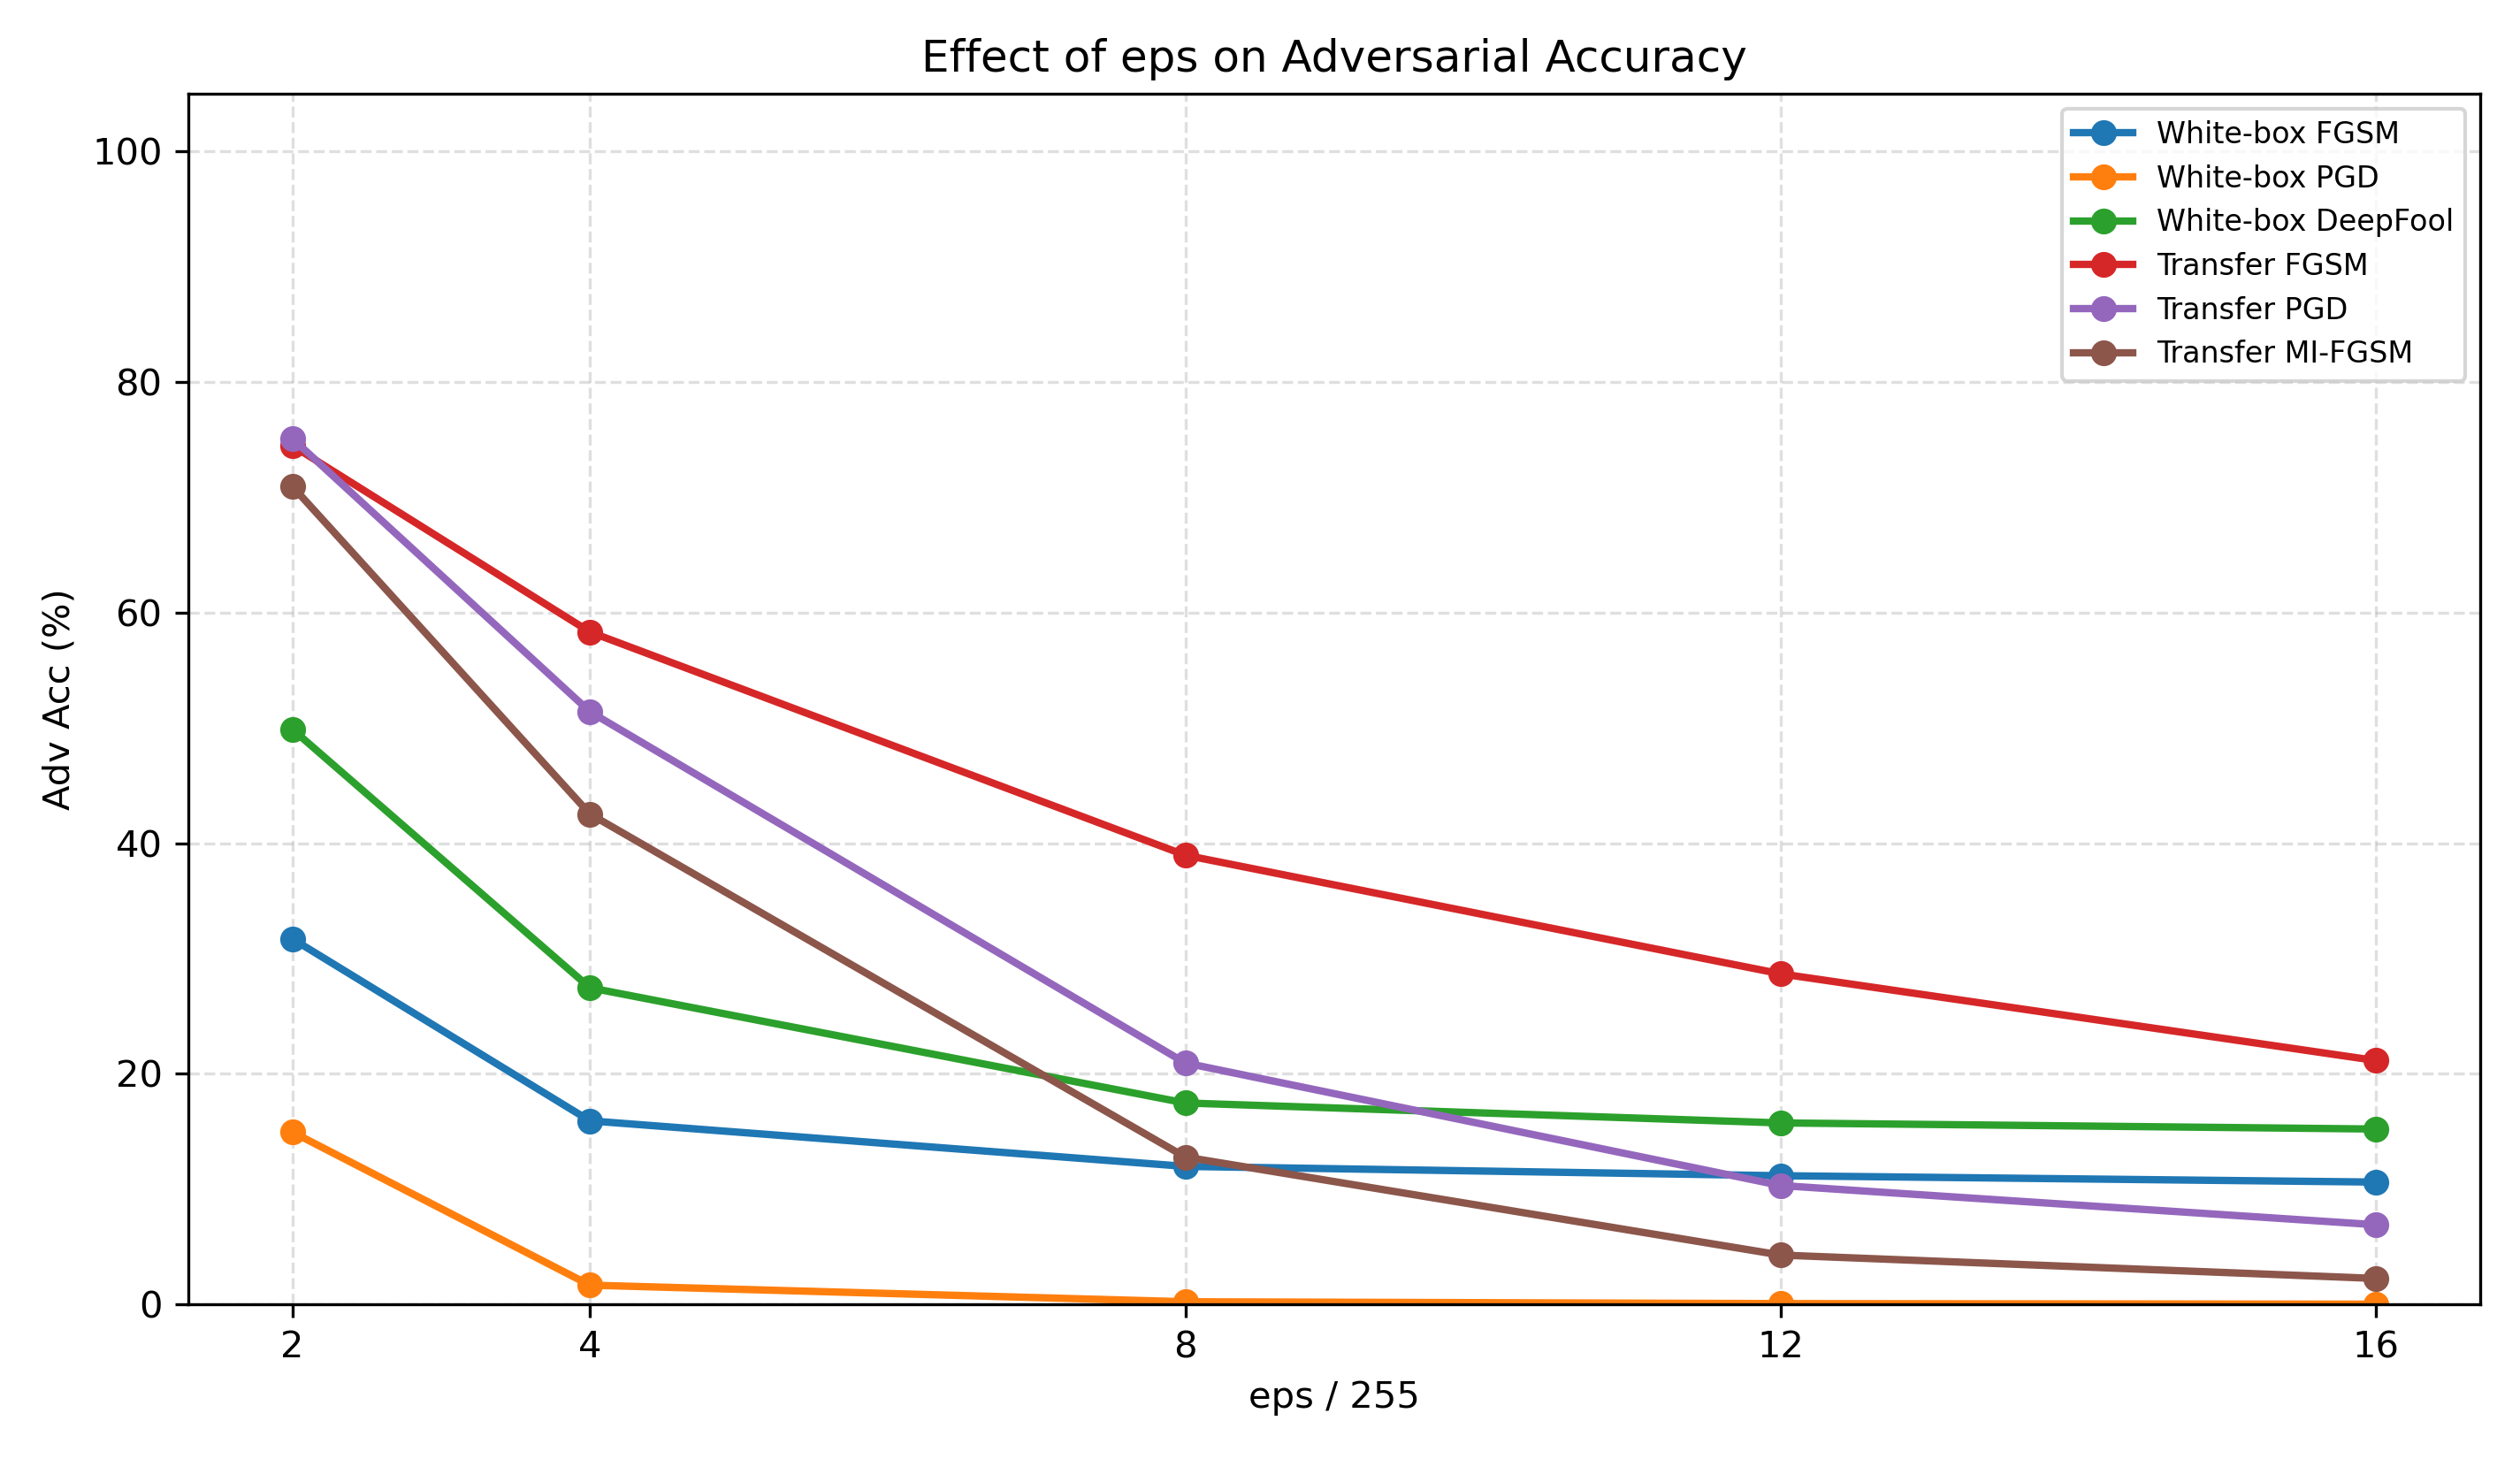
\includegraphics[width=\textwidth]{figure/eps2.png}
        \caption{eps 对对抗样本准确率 Adv Acc 的影响}
        \label{fig:eps_adv_acc}
    \end{subfigure}

    \caption{扰动大小 eps 对攻击效果的影响}
    \label{fig:eps}
\end{figure}
\subsection{迭代次数 steps 对攻击效果的影响}

本实验固定 $\epsilon=8/255$，$\alpha=2/255$，改变 steps，测试不同迭代型攻击方法的效果。FGSM 为单步攻击，因此不参与 steps 敏感性分析。

\begin{table}[H]
    \centering
    \caption{迭代次数 steps 对攻击效果的影响}
    \resizebox{\textwidth}{!}{
    \begin{tabular}{ccccccc}
        \toprule
        攻击类型 & 攻击方法 & steps=1 & steps=3 & steps=5 & steps=10 & steps=20 \\
        \midrule
        白盒攻击 & PGD & 24.04 / 73.74 & 3.88 / 95.76 & 1.48 / 98.38 & 0.24 / 99.74 & 0.07 / 99.92 \\
        白盒攻击 & DeepFool & 72.97 / 23.49 & 30.74 / 71.97 & 20.75 / 83.02 & 17.45 / 86.64 & 17.31 / 86.83 \\
        迁移攻击 & PGD & 68.13 / 25.67 & 39.70 / 56.67 & 27.47 / 69.99 & 20.21 / 77.92 & 20.18 / 77.99 \\
        迁移攻击 & MI-FGSM & 74.49 / 18.66 & 28.60 / 68.76 & 14.57 / 84.08 & 12.78 / 86.06 & 12.92 / 85.90 \\
        迁移攻击 & DeepFool & 89.46 / 2.56 & 89.18 / 2.86 & 89.17 / 2.87 & 89.17 / 2.87 & 89.17 / 2.87 \\
        \bottomrule
    \end{tabular}
    }
    \label{tab:steps_sensitivity}
\end{table}

表~\ref{tab:steps_sensitivity} 中单元格格式为 ``Adv Acc / ASR''，单位均为百分比。可以看出，随着迭代次数 steps 增加，PGD、DeepFool 和 MI-FGSM 的攻击成功率整体上升，对抗样本准确率整体下降。其中白盒 PGD 对迭代次数最敏感，在 steps=3 时 ASR 已达到 95.76\%，steps=10 后基本趋于饱和。

\begin{figure}[H]
    \centering

    \begin{subfigure}[b]{0.48\textwidth}
        \centering
        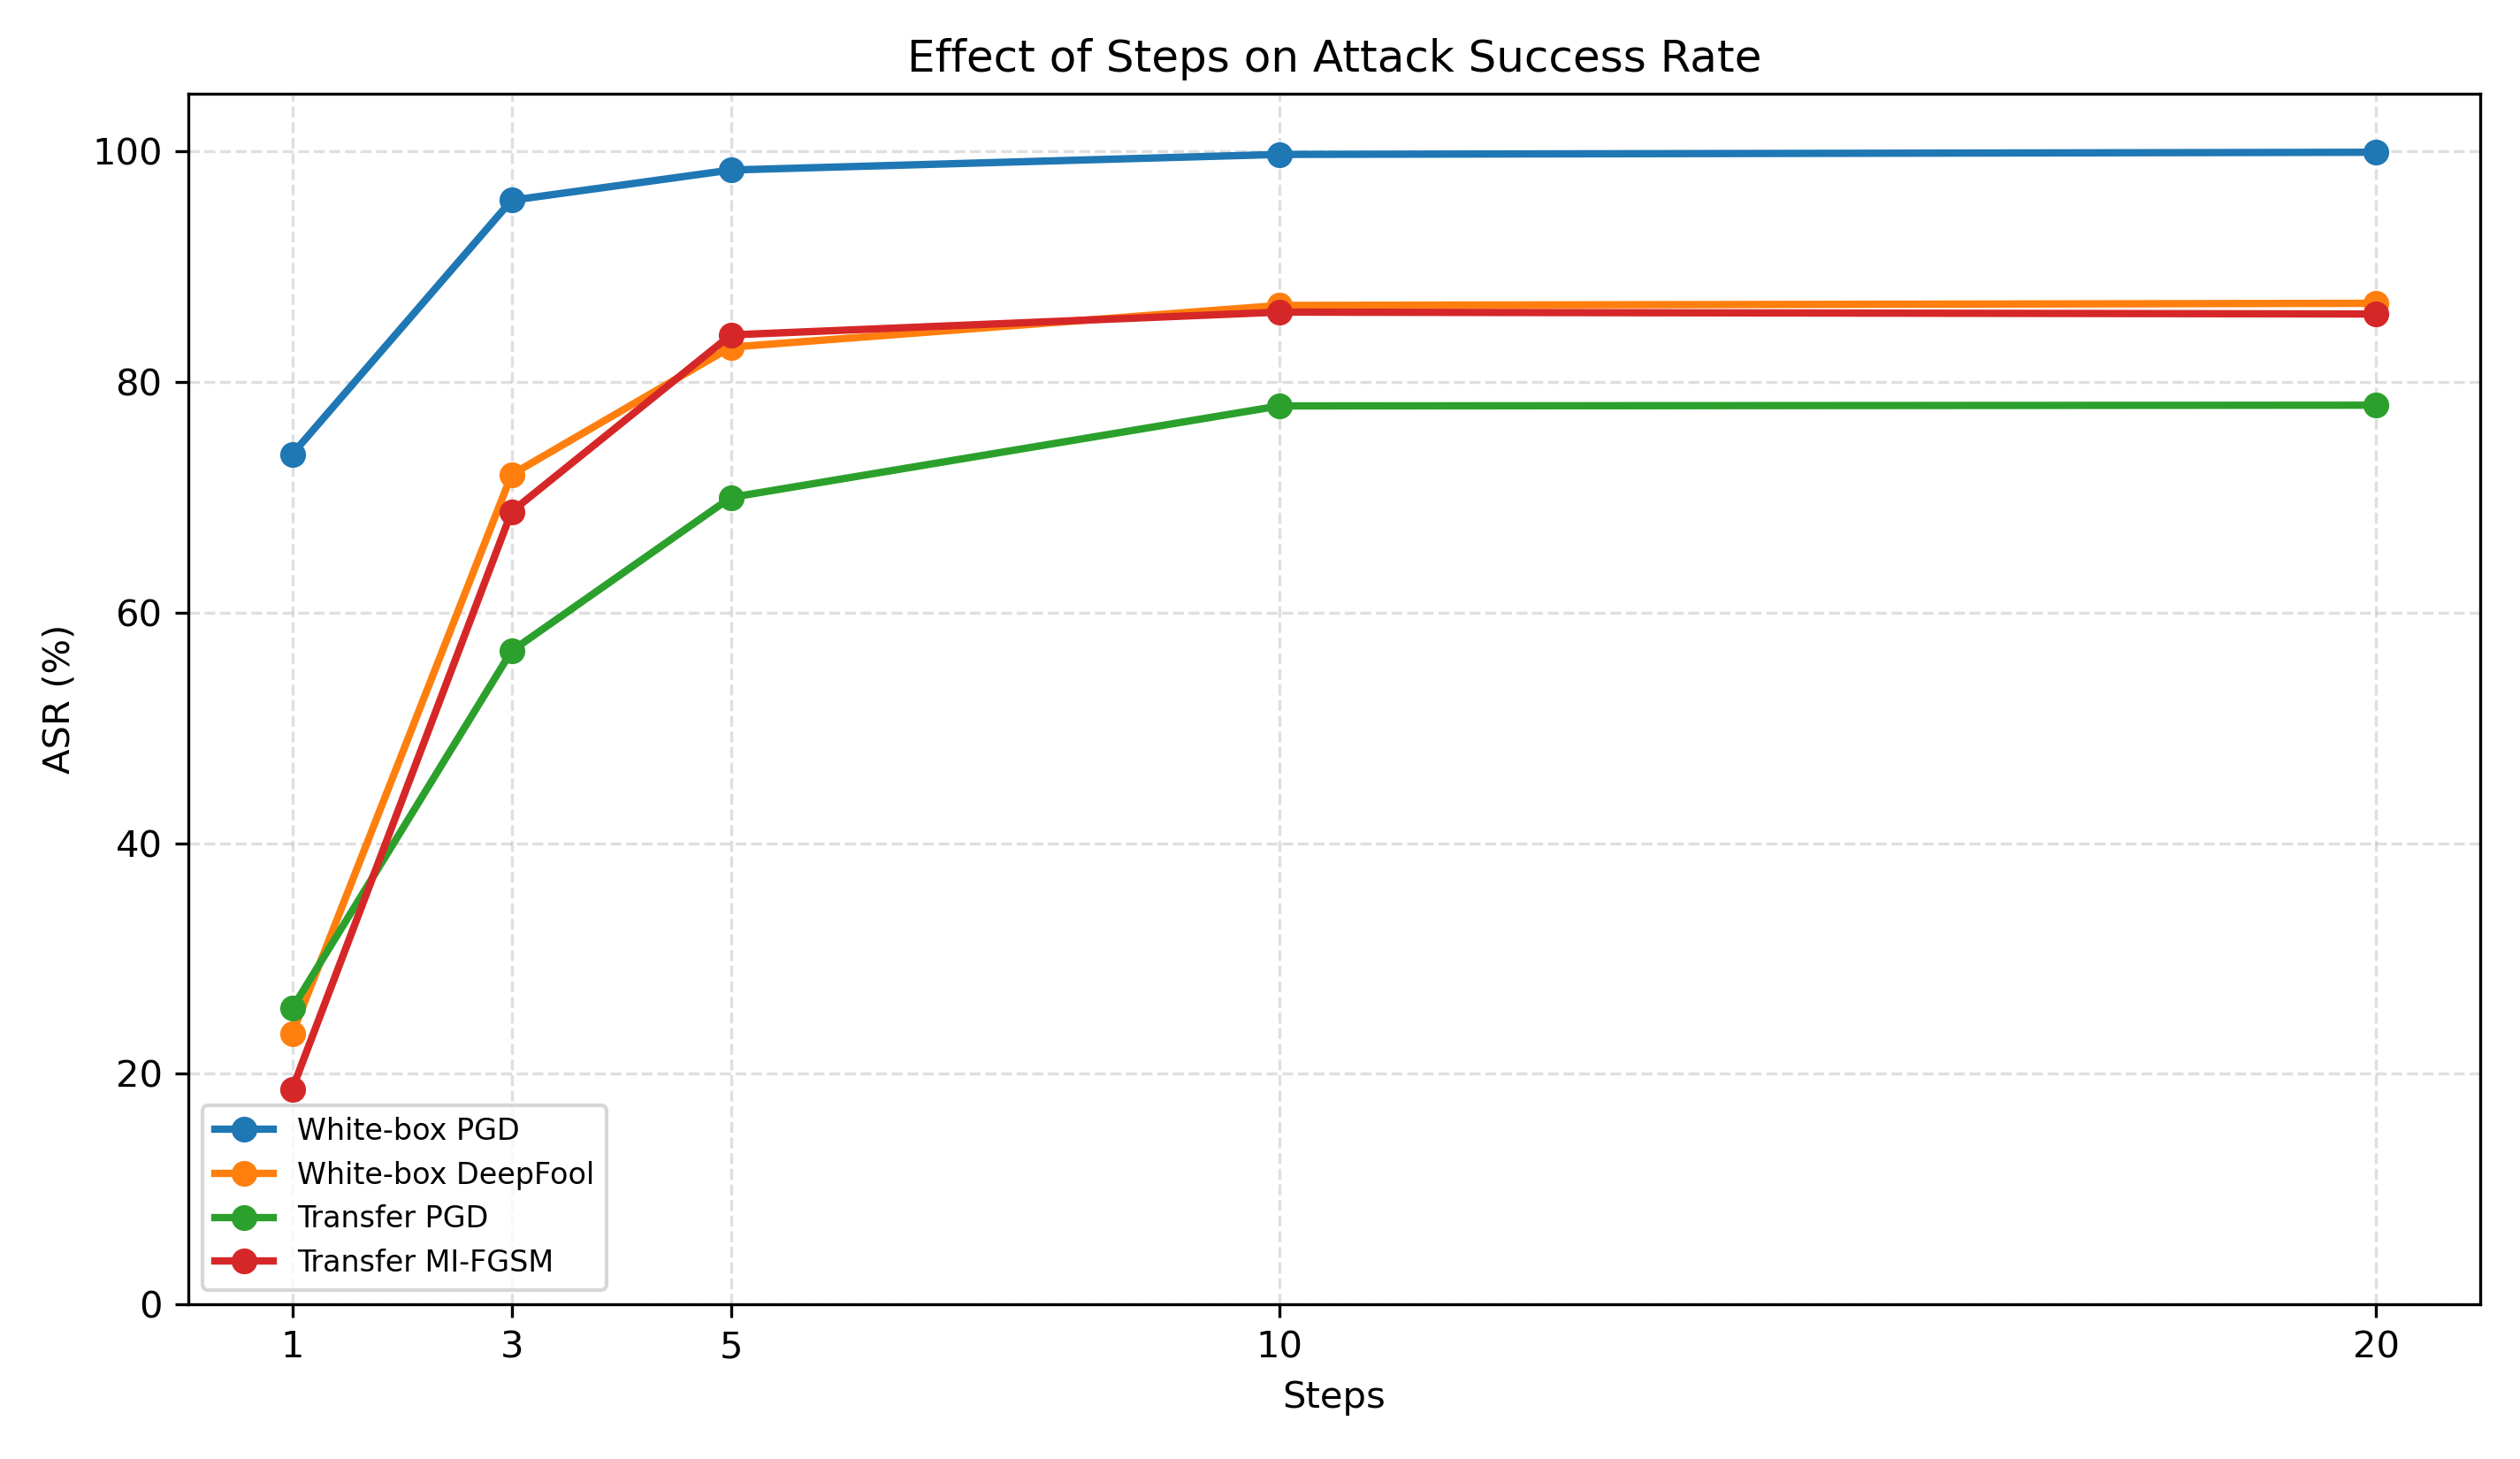
\includegraphics[width=\textwidth]{figure/steps1.png}
        \caption{steps 对攻击成功率 ASR 的影响}
        \label{fig:steps_asr}
    \end{subfigure}
    \hfill
    \begin{subfigure}[b]{0.48\textwidth}
        \centering
        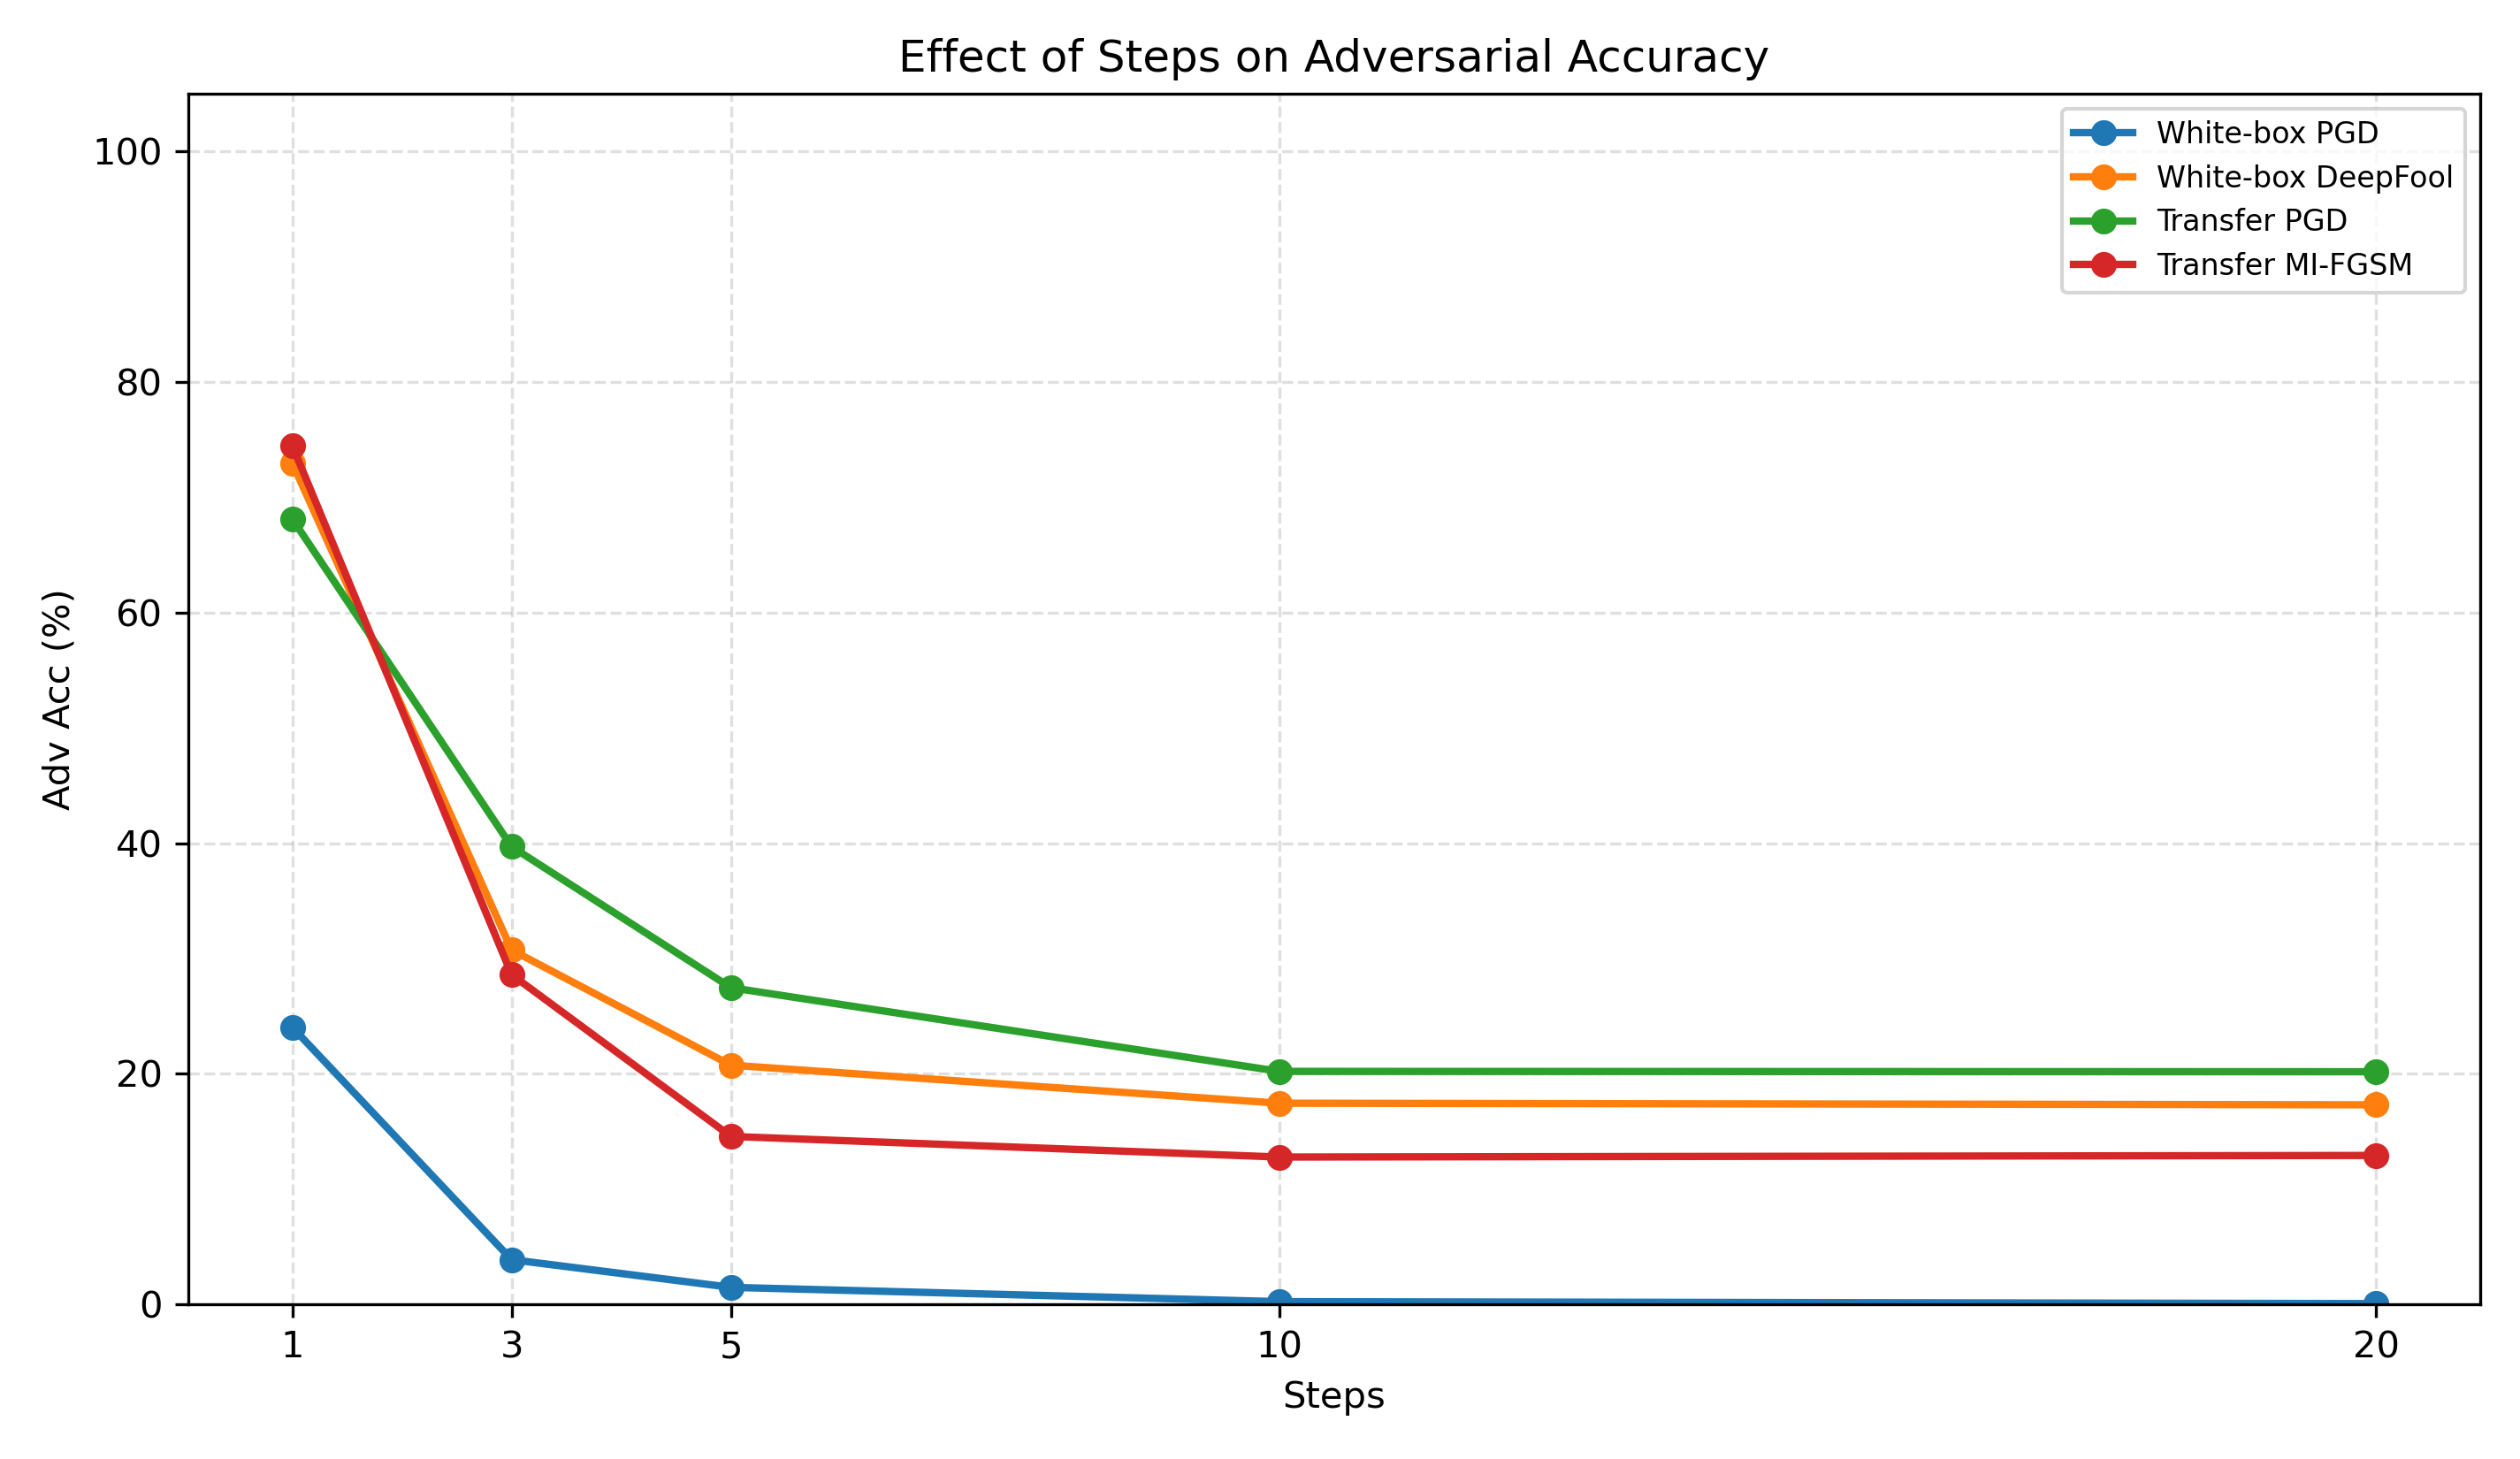
\includegraphics[width=\textwidth]{figure/steps2.png}
        \caption{steps 对对抗样本准确率 Adv Acc 的影响}
        \label{fig:steps_adv_acc}
    \end{subfigure}

    \caption{迭代次数 steps 对攻击效果的影响}
    \label{fig:steps}
\end{figure}

\subsection{防御实验与自适应评估}

\subsubsection{防御方法介绍}

本实验采用两类防御方法：输入预处理防御和对抗训练防御。输入预处理防御的核心思想是在对抗样本输入模型之前，对图像进行简单处理，削弱扰动对模型判断的影响。对抗训练防御的核心思想是在训练过程中主动加入对抗样本，使模型提前学习攻击样本的特征，从而提升模型对对抗扰动的适应能力。

\begin{table}[H]
    \centering
    \caption{防御方法概述}
    \resizebox{\textwidth}{!}{
    \begin{tabular}{p{3cm}p{4cm}p{4cm}p{4cm}}
        \toprule
        防御类型 & 防御方法 & 核心思想 & 局限 \\
        \midrule
        输入预处理防御 & 位深压缩、JPEG 压缩 & 在输入模型前削弱扰动 & 对强攻击防御有限，可能降低图像质量 \\
        对抗训练防御 & FGSM 对抗训练、PGD 对抗训练 & 训练时加入对抗样本 & 训练成本更高，可能降低干净样本准确率 \\
        \bottomrule
    \end{tabular}
    }
    \label{tab:defense_methods}
\end{table}

\subsubsection{输入预处理防御结果}

输入预处理防御主要包括 JPEG 压缩和位深压缩。JPEG 压缩利用有损压缩去除部分高频扰动；位深压缩通过降低图像像素表示精度来削弱微小扰动。

\begin{table}[H]
    \centering
    \caption{输入预处理防御实验结果}
    \begin{tabular}{ccccc}
        \toprule
        防御方法 & 攻击方法 & Clean Acc & Adv Acc & ASR \\
        \midrule
        JPEG 压缩 & FGSM & 84.04\% & 27.20\% & 67.84\% \\
        位深压缩 & FGSM & 91.33\% & 12.13\% & 86.74\% \\
        JPEG 压缩 & PGD & 84.04\% & 17.79\% & 78.87\% \\
        位深压缩 & PGD & 91.33\% & 0.26\% & 99.72\% \\
        JPEG 压缩 & DeepFool & 84.04\% & 79.83\% & 5.45\% \\
        位深压缩 & DeepFool & 91.33\% & 71.31\% & 21.92\% \\
        \bottomrule
    \end{tabular}
    \label{tab:preprocess_defense}
\end{table}

由表~\ref{tab:preprocess_defense} 可见，JPEG 压缩会降低干净样本准确率，但对 DeepFool 有一定缓解作用；位深压缩基本保持干净样本准确率，但面对 PGD 等强梯度攻击时防御效果有限。

\subsubsection{FGSM 对抗训练结果}

对抗训练是一种常见的鲁棒性提升方法。普通训练只使用干净样本，而对抗训练在训练阶段主动加入对抗样本，使模型学习在扰动条件下仍然输出正确类别。

\begin{table}[H]
    \centering
    \caption{FGSM 单步对抗训练防御结果}
    \resizebox{\textwidth}{!}{
    \begin{tabular}{cccccc}
        \toprule
        防御方法 & 攻击类型 & 攻击方法 & Clean Acc & Adv Acc & ASR \\
        \midrule
        FGSM 对抗训练 & 白盒攻击 & FGSM & 83.33\% & 69.10\% & 23.57\% \\
        FGSM 对抗训练 & 白盒攻击 & PGD & 83.33\% & 0.05\% & 99.94\% \\
        FGSM 对抗训练 & 白盒攻击 & DeepFool & 83.33\% & 26.77\% & 77.80\% \\
        FGSM 对抗训练 & 迁移攻击 & FGSM & 83.33\% & 67.84\% & 21.86\% \\
        FGSM 对抗训练 & 迁移攻击 & PGD & 83.33\% & 71.53\% & 18.06\% \\
        FGSM 对抗训练 & 迁移攻击 & MI-FGSM & 83.33\% & 63.79\% & 26.15\% \\
        FGSM 对抗训练 & 迁移攻击 & DeepFool & 83.33\% & 82.38\% & 1.56\% \\
        FGSM 对抗训练 & 黑盒攻击 & SPSA & 84.40\% & 42.70\% & 50.00\% \\
        \bottomrule
    \end{tabular}
    }
    \label{tab:fgsm_adv_training}
\end{table}

FGSM 对抗训练显著提升了模型对 FGSM 和部分迁移攻击的鲁棒性，但面对白盒 PGD 强攻击时几乎被完全攻破，PGD 攻击成功率达到 99.94\%。这说明单步对抗训练对强多步攻击防御能力有限。

\subsubsection{PGD 对抗训练结果}

为了进一步提升模型对强攻击的鲁棒性，本文采用 PGD 对抗训练作为最终防御方案。

\begin{table}[H]
    \centering
    \caption{PGD 对抗训练最终版防御结果}
    \resizebox{\textwidth}{!}{
    \begin{tabular}{cccccc}
        \toprule
        防御方法 & 攻击类型 & 攻击方法 & Clean Acc & Adv Acc & ASR \\
        \midrule
        PGD 对抗训练 & 白盒攻击 & FGSM & 83.37\% & 47.48\% & 43.06\% \\
        PGD 对抗训练 & 白盒攻击 & PGD & 83.37\% & 35.53\% & 57.38\% \\
        PGD 对抗训练 & 白盒攻击 & DeepFool & 83.37\% & 68.77\% & 26.47\% \\
        PGD 对抗训练 & 迁移攻击 & FGSM & 83.37\% & 79.20\% & 5.34\% \\
        PGD 对抗训练 & 迁移攻击 & PGD & 83.37\% & 80.91\% & 3.15\% \\
        PGD 对抗训练 & 迁移攻击 & MI-FGSM & 83.37\% & 79.81\% & 4.61\% \\
        PGD 对抗训练 & 迁移攻击 & DeepFool & 83.37\% & 83.18\% & 0.25\% \\
        PGD 对抗训练 & 黑盒攻击 & SPSA & 84.40\% & 75.70\% & 10.31\% \\
        \bottomrule
    \end{tabular}
    }
    \label{tab:pgd_adv_training}
\end{table}

与 FGSM 对抗训练相比，PGD 对抗训练在白盒 PGD 攻击下提升最明显。PGD Adv Acc 从 0.05\% 提升到 35.53\%，ASR 从 99.94\% 降低到 57.38\%。同时，在迁移攻击和黑盒 SPSA 攻击下，PGD 对抗训练也表现出更强稳定性。

\begin{figure}[H]
    \centering
    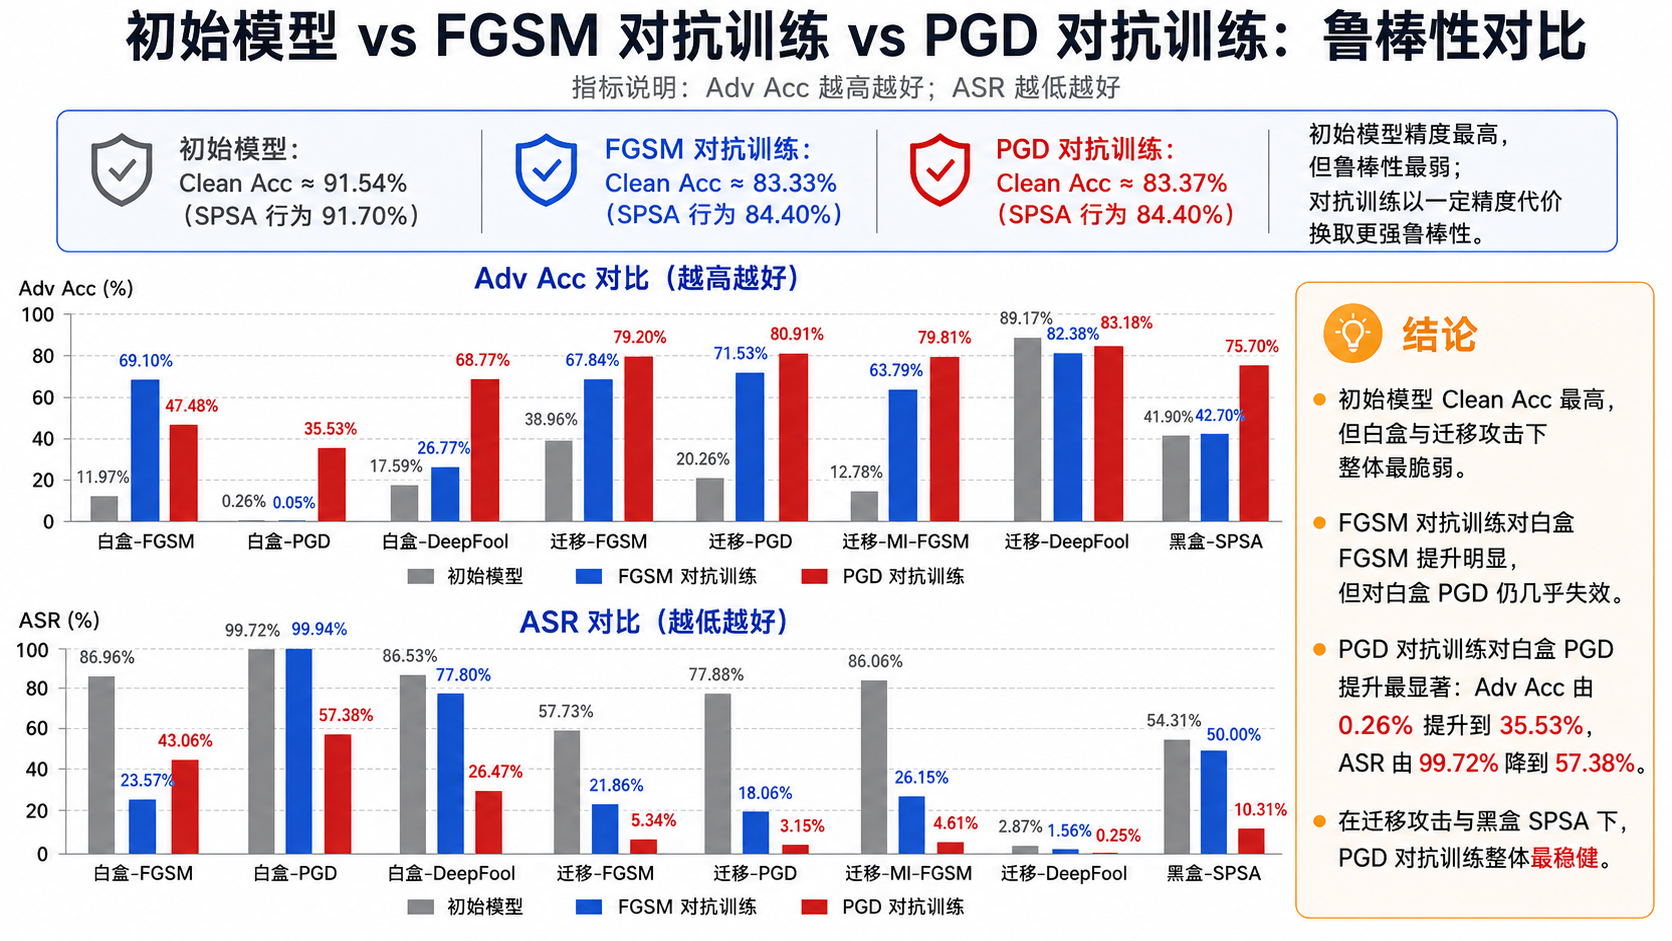
\includegraphics[width=0.95\textwidth]{figure/鲁棒性.png}
    \caption{初始模型、FGSM 对抗训练与 PGD 对抗训练鲁棒性对比}
    \label{fig:defense_compare}
\end{figure}

\subsubsection{BPDA 自适应攻击评估}

在输入预处理防御中，JPEG 压缩和位深压缩等操作往往不可导或梯度不稳定。如果直接使用普通梯度攻击，攻击可能因为无法正确反向传播而被削弱，从而导致防御效果被高估。为避免这一问题，本实验采用 BPDA 自适应攻击进行评估。BPDA 的核心思想是前向传播时使用真实预处理操作，反向传播时使用近似恒等映射代替不可导部分。

\begin{table}[H]
    \centering
    \caption{BPDA 自适应攻击评估结果}
    \begin{tabular}{ccccc}
        \toprule
        防御方法 & 自适应攻击方法 & Clean Acc & Adv Acc & ASR \\
        \midrule
        JPEG 压缩 & PGD + BPDA & 84.04\% & 2.32\% & 97.24\% \\
        位深压缩 & PGD + BPDA & 91.33\% & 0.29\% & 99.68\% \\
        \bottomrule
    \end{tabular}
    \label{tab:bpda}
\end{table}

由表~\ref{tab:bpda} 可知，在 BPDA 自适应攻击下，JPEG 压缩和位深压缩几乎都被重新攻破。这说明简单输入预处理方法存在梯度遮蔽风险，普通攻击下看似有效，但在自适应攻击下防御能力明显不足。

\section{结果分析}
\subsection{定量指标分析}

从定量结果来看，攻击、防御与自适应评估之间呈现出较为清晰的规律。首先，在攻击侧，白盒 PGD 对普通模型破坏最强，说明多步梯度投影仍然是当前实验设定下最具代表性的强攻击；在迁移攻击中，MI-FGSM 的攻击成功率最高，体现了动量项对跨模型迁移性的增强作用。其次，在防御侧，JPEG 压缩与位深压缩只能对部分攻击形成有限缓解，尤其难以抵抗 PGD 这类强梯度攻击；而 PGD 对抗训练在白盒、迁移和黑盒场景下都能保持更高的 Adv Acc，是本实验中综合效果最好的防御方案。最后，BPDA 结果表明预处理防御在自适应攻击下几乎全部失效，这说明仅依赖输入端变换并不能建立可靠鲁棒性。

\subsection{t-SNE 特征分布可视化}

为了进一步分析对抗样本为什么会导致模型误分类，本实验使用 t-SNE 方法对模型提取的高维特征进行降维可视化。具体做法是：首先将正常样本和对应的对抗样本输入模型，提取模型中间层或倒数层特征；然后使用 t-SNE 将高维特征映射到二维空间；最后比较正常样本和对抗样本在特征空间中的分布差异。

\begin{figure}[H]
    \centering

    \begin{subfigure}[b]{0.95\textwidth}
        \centering
        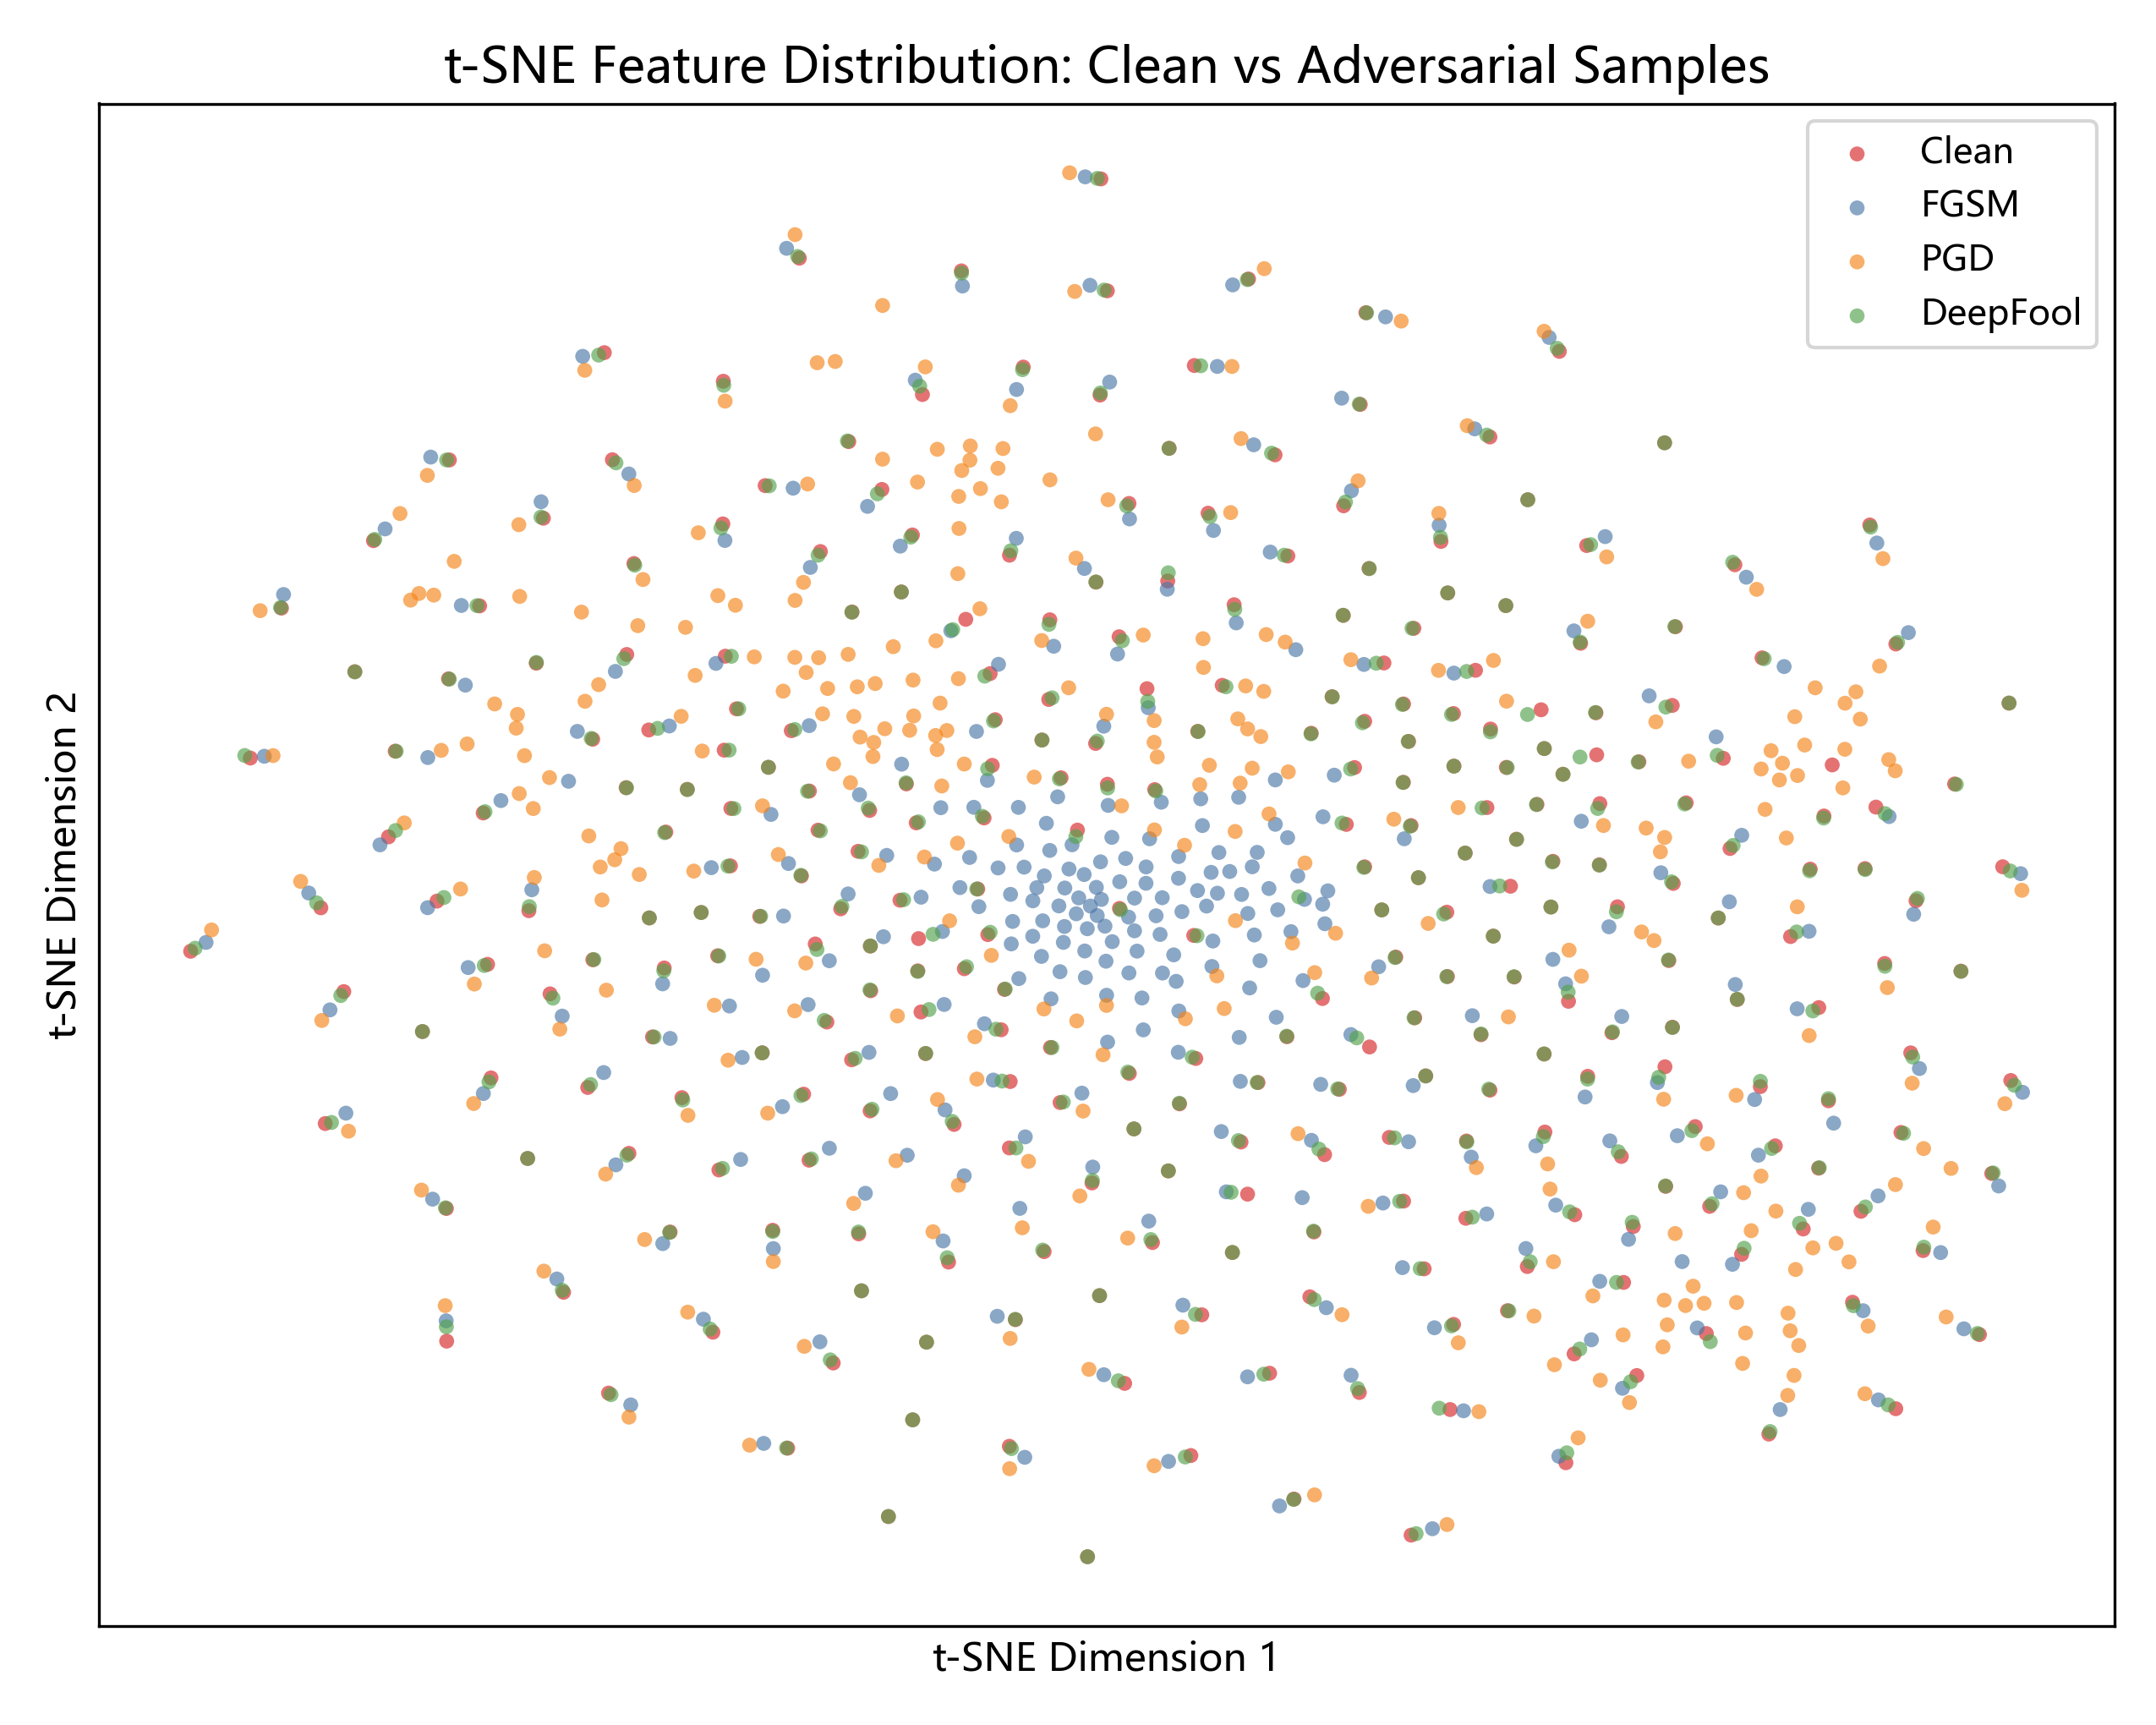
\includegraphics[width=\textwidth]{figure/tsne.png}
        \caption{Clean 样本与多种对抗样本的 t-SNE 总体分布}
        \label{fig:tsne_overall}
    \end{subfigure}

    \vspace{0.8em}

    \begin{subfigure}[b]{0.95\textwidth}
        \centering
        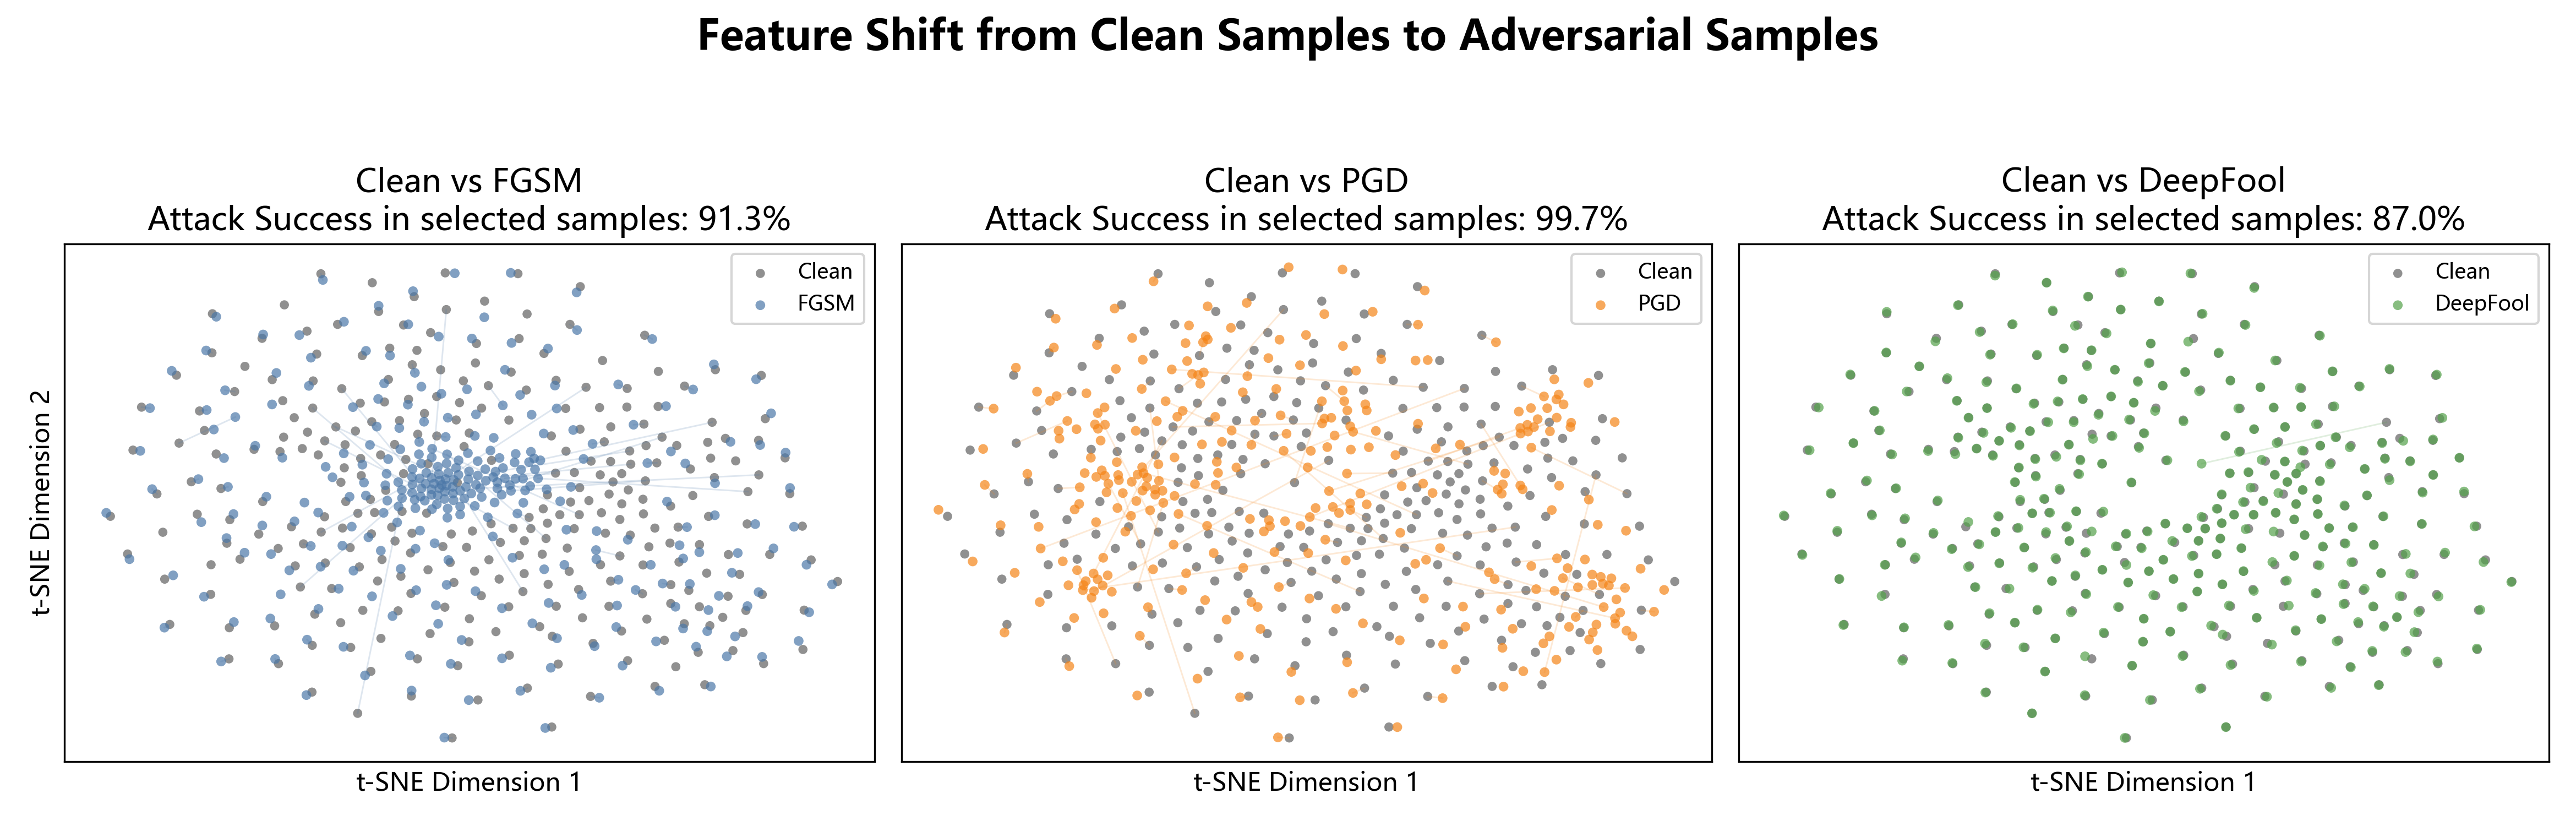
\includegraphics[width=\textwidth]{figure/tsne2.png}
        \caption{Clean 样本与不同攻击样本的特征偏移对比}
        \label{fig:tsne_each_attack}
    \end{subfigure}

    \caption{Clean 样本与对抗样本的 t-SNE 特征分布可视化}
    \label{fig:tsne}
\end{figure}

从 t-SNE 可视化结果可以观察到，正常样本通常会按照类别形成相对集中的特征簇，而对抗样本在加入微小扰动后，其特征位置会发生明显偏移。部分对抗样本会从原类别特征簇附近移动到其他类别区域，从而导致模型预测结果发生错误。这说明对抗扰动虽然在像素空间中很小，但会显著改变模型内部特征表示，使样本在特征空间中靠近或进入错误类别区域。

\subsection{对抗样本差异可视化}

为了更直观地观察对抗样本与原图之间的差异，本文将原图、放大后的扰动图和对抗样本进行并列展示。扰动图通过将 $x_{\mathrm{adv}} - x$ 放大若干倍后可视化得到。

\begin{figure}[H]
    \centering
    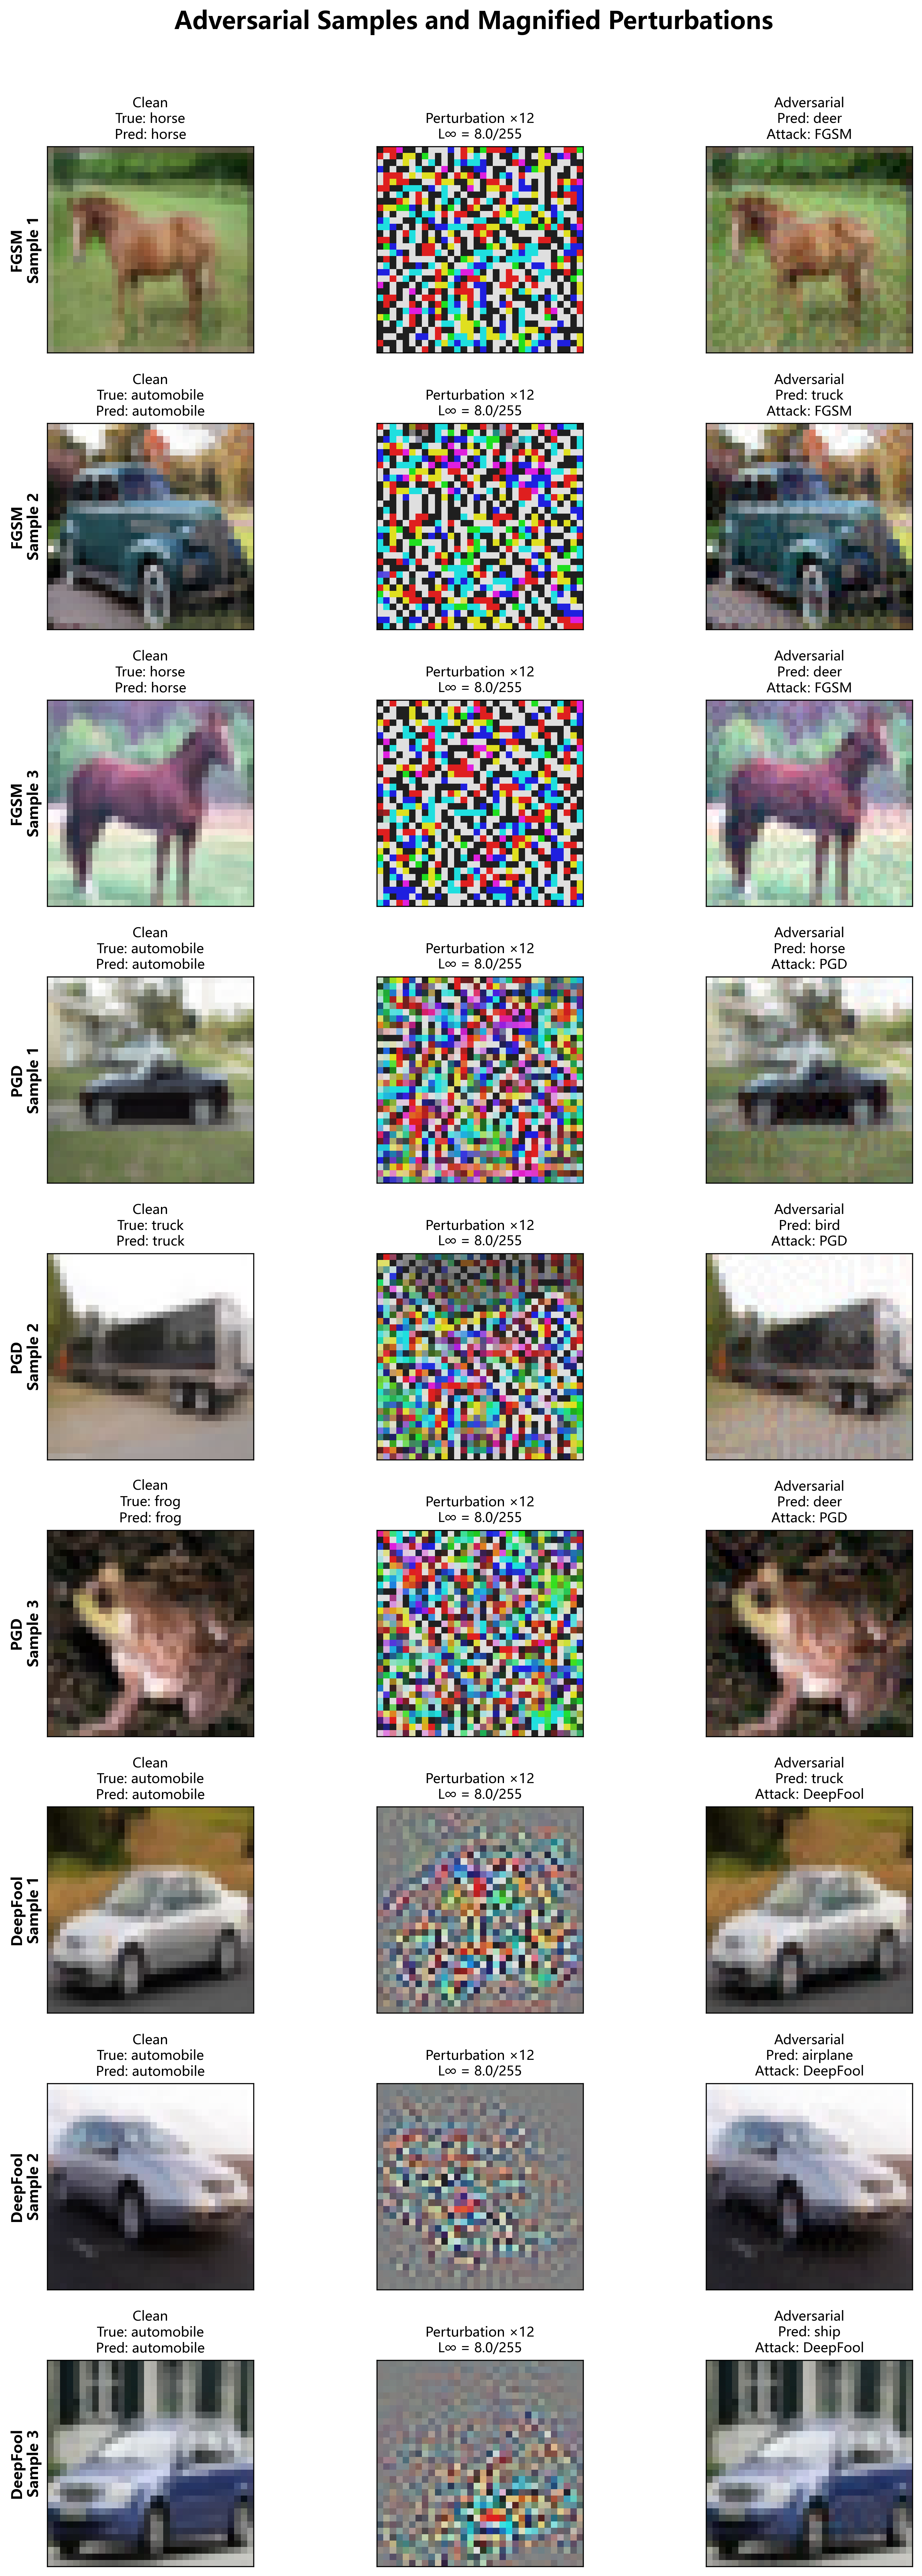
\includegraphics[width=0.5\textwidth]{figure/adv_diff_examples.png}
    \caption{原图、放大扰动与对抗样本可视化}
    \label{fig:adv_diff}
\end{figure}
该可视化结果表明，对抗扰动在原图和对抗样本之间肉眼差异较小，但经过放大后可以看到扰动通常呈现高频噪声形态。尽管像素变化幅度受限于 $8/255$，但该扰动仍然能够显著改变模型预测结果。

\subsection{最脆弱类别分析}

本实验进一步统计 FGSM、PGD 和 DeepFool 三种攻击下模型最容易被攻破的类别。结果如表~\ref{tab:fragile_classes} 所示。

\begin{table}[H]
    \centering
    \caption{最脆弱类别 Top-5}
    \begin{tabular}{ccccc}
        \toprule
        排名 & 类别 & Clean 正确样本数 & 攻击成功总次数 & 平均 ASR \\
        \midrule
        1 & cat & 834 & 2392 & 95.60\% \\
        2 & frog & 937 & 2631 & 93.60\% \\
        3 & horse & 928 & 2584 & 92.82\% \\
        4 & dog & 877 & 2439 & 92.70\% \\
        5 & bird & 878 & 2434 & 92.41\% \\
        \bottomrule
    \end{tabular}
    \label{tab:fragile_classes}
\end{table}

从表~\ref{tab:fragile_classes} 可以看出，cat、frog、horse、dog 和 bird 等类别的平均攻击成功率最高，说明模型在这些类别上的特征判别边界相对更脆弱。这些类别本身具有较强的外观变化和类间相似性，因此更容易受到对抗扰动影响。

\subsection{最脆弱样本分析}

表~\ref{tab:fragile_samples} 给出了按照 margin drop 排序得到的最脆弱样本。Margin drop 表示攻击前后真实类别 logit 的下降幅度，数值越大，说明攻击对模型真实类别判断的破坏越明显。

\begin{table}[H]
    \centering
    \caption{最脆弱样本 Top-10}
    \resizebox{\textwidth}{!}{
    \begin{tabular}{ccccccc}
        \toprule
        排名 & 样本编号 & 攻击方法 & 真实类别 & 原始预测 & 攻击后预测 & Margin Drop \\
        \midrule
        1 & 594 & PGD & automobile & automobile & horse & 39.80 \\
        2 & 2907 & PGD & truck & truck & bird & 38.76 \\
        3 & 5807 & PGD & frog & frog & deer & 38.61 \\
        4 & 7876 & DeepFool & automobile & automobile & truck & 38.03 \\
        5 & 7273 & PGD & deer & deer & bird & 37.95 \\
        6 & 4978 & PGD & automobile & automobile & bird & 37.75 \\
        7 & 5347 & PGD & automobile & automobile & cat & 37.71 \\
        8 & 9813 & PGD & automobile & automobile & dog & 37.70 \\
        9 & 6891 & PGD & truck & truck & bird & 37.49 \\
        10 & 6317 & PGD & truck & truck & bird & 37.44 \\
        \bottomrule
    \end{tabular}
    }
    \label{tab:fragile_samples}
\end{table}

可以看到，最脆弱样本中 PGD 攻击占比较高，且多数样本的 $L_\infty$ 扰动均达到 $8/255$ 上限，说明 PGD 能够在限制扰动范围内显著降低模型对真实类别的判别置信度。

\section{结论与展望}

本文基于 CIFAR-10 数据集，围绕对抗样本攻击与防御展开实验研究，重点分析了白盒攻击、黑盒攻击和迁移攻击在不同模型和防御方法下的表现。

首先，在攻击实验中，白盒 PGD 表现出最强攻击能力。对于初始模型，PGD 攻击后 Adv Acc 仅为 0.26\%，ASR 达到 99.72\%，说明普通分类模型在强白盒攻击下非常脆弱。其次，在迁移攻击中，MI-FGSM 表现最好。它在 Model A 上生成对抗样本后迁移到 Model B，仍然能够取得较高攻击成功率，说明动量机制可以增强对抗样本的跨模型迁移能力。

在防御实验中，输入预处理方法实现简单，但整体防御能力有限。JPEG 压缩对 DeepFool 有一定缓解作用，位深压缩对干净样本准确率影响较小，但二者都难以抵抗 PGD 强攻击。进一步使用 BPDA 自适应攻击后，JPEG 压缩和位深压缩几乎被重新攻破，说明简单输入预处理存在梯度遮蔽风险，不能作为可靠的强鲁棒防御方法。

最后，对抗训练能够显著提升模型鲁棒性。其中 FGSM 对抗训练对白盒 FGSM 和部分迁移攻击有效，但面对白盒 PGD 仍然不足；PGD 对抗训练综合效果最好，在白盒攻击、迁移攻击和黑盒 SPSA 下均表现出更强稳定性。因此，PGD 对抗训练是本实验中最有效的鲁棒性提升方法。

\subsection{不足与改进方向}

虽然本实验完成了多种对抗攻击与防御方法的实现和对比，但仍然存在一些不足。

首先，在防御方法方面，本实验主要采用输入预处理防御和对抗训练防御。其中输入预处理方法实现简单，但在 BPDA 自适应攻击下防御效果明显下降，说明其鲁棒性有限。

其次，在对抗训练方面，FGSM 对抗训练对单步攻击有一定防御效果，但对白盒 PGD 这类强多步攻击防御不足。PGD 对抗训练虽然综合效果更好，但会牺牲一定干净样本准确率，并且训练成本更高。

第三，在攻击方法方面，本文已经实现 FGSM、PGD、DeepFool、MI-FGSM 和 SPSA，但还可以进一步加入 CW Attack、AutoAttack 等更严格的攻击方法，对模型鲁棒性进行更全面评估。

最后，本实验只在 CIFAR-10 数据集上进行验证，后续可以扩展到更大规模数据集和更复杂模型，例如 CIFAR-100、Tiny-ImageNet 或更深层 CNN / Transformer 结构，以进一步验证攻击与防御方法的泛化能力。

\begin{table}[H]
    \centering
    \caption{不足与改进方向}
    \resizebox{\textwidth}{!}{
    \begin{tabular}{ccc}
        \toprule
        不足 & 说明 & 改进方向 \\
        \midrule
        输入预处理防御有限 & BPDA 后几乎被攻破 & 引入更强鲁棒防御方法 \\
        FGSM 对抗训练不足 & 难以防御白盒 PGD & 使用 PGD 对抗训练或混合攻击训练 \\
        攻击方法仍可扩展 & 当前未加入 AutoAttack、CW & 增加更严格攻击评估 \\
        数据集规模较小 & 仅在 CIFAR-10 上验证 & 扩展到 CIFAR-100、Tiny-ImageNet \\
        \bottomrule
    \end{tabular}
    }
    \label{tab:limitations}
\end{table}

% =========================================================
\begin{thebibliography}{99}

\bibitem{goodfellow2014}
I. J. Goodfellow, J. Shlens, and C. Szegedy,
``Explaining and Harnessing Adversarial Examples,''
International Conference on Learning Representations, 2015.

\bibitem{madry2017}
A. Madry, A. Makelov, L. Schmidt, D. Tsipras, and A. Vladu,
``Towards Deep Learning Models Resistant to Adversarial Attacks,''
International Conference on Learning Representations, 2018.

\bibitem{deepfool}
S.-M. Moosavi-Dezfooli, A. Fawzi, and P. Frossard,
``DeepFool: A Simple and Accurate Method to Fool Deep Neural Networks,''
IEEE Conference on Computer Vision and Pattern Recognition, 2016.

\bibitem{mifgsm}
Y. Dong, F. Liao, T. Pang, H. Su, J. Zhu, X. Hu, and J. Li,
``Boosting Adversarial Attacks with Momentum,''
IEEE Conference on Computer Vision and Pattern Recognition, 2018.

\bibitem{spsa}
J. C. Spall,
``Multivariate Stochastic Approximation Using a Simultaneous Perturbation Gradient Approximation,''
IEEE Transactions on Automatic Control, 1992.

\bibitem{bpda}
A. Athalye, N. Carlini, and D. Wagner,
``Obfuscated Gradients Give a False Sense of Security: Circumventing Defenses to Adversarial Examples,''
International Conference on Machine Learning, 2018.

\end{thebibliography}

\section{成员分工}

\subsection*{金纪勇（贡献度：30\%）}
\begin{enumerate}
    \item 项目总体方案设计与技术路线制定；
    \item SimpleCNN 与 ResNet18 模型训练；
    \item FGSM、PGD、MI-FGSM、DeepFool、SPSA 等攻击算法实现；
    \item JPEG Compression、Feature Squeezing、BPDA 防御算法实现；
    \item FGSM 与 PGD 对抗训练模型设计与实现；
    \item EPS 扰动大小和 PGD 迭代次数敏感性实验；
    \item 对抗样本可视化、t-SNE 特征分析、脆弱类别分析；
    \item 实验结果统计分析与图表绘制；
    \item GitHub 项目整理、README 编写；
    \item 实验报告与 PPT 制作。
\end{enumerate}

\subsection*{周杨（贡献度：25\%）}
\begin{enumerate}
    \item CIFAR-10 数据集整理与预处理；
    \item 模型训练流程调试；
    \item 攻击与防御实验运行；
    \item 实验数据统计与整理；
    \item 协助实验结果验证与分析。
\end{enumerate}

\subsection*{程湜（贡献度：15\%）}
\begin{enumerate}
    \item 攻击效果评估模块实现；
    \item 白盒攻击实验测试；
    \item 迁移攻击实验测试；
    \item 黑盒攻击实验测试；
    \item EPS 敏感性实验；
    \item Steps 敏感性实验；
    \item 实验结果汇总与统计图制作。
\end{enumerate}

\subsection*{廖苒希（贡献度：15\%）}
\begin{enumerate}
    \item 对抗样本可视化；
    \item t-SNE 特征分布分析；
    \item 扰动放大可视化；
    \item 脆弱类别统计分析；
    \item 实验图片整理；
    \item 协助实验结果分析。
\end{enumerate}

\subsection*{朱子淼（贡献度：15\%）}
\begin{enumerate}
    \item 项目文档整理；
    \item README 文档编写与维护；
    \item PPT 制作；
    \item 实验报告排版；
    \item GitHub 项目维护；
    \item 项目成果展示与材料整理。
\end{enumerate}

\begin{table}[H]
    \centering
    \caption{贡献度统计}
    \begin{tabular}{cc}
        \toprule
        成员 & 贡献度 \\
        \midrule
        金纪勇 & 30\% \\
        周杨 & 25\% \\
        程湜 & 15\% \\
        廖苒希 & 15\% \\
        朱子淼 & 15\% \\
        \bottomrule
    \end{tabular}
\end{table}

本项目由以上五位成员共同完成。各成员根据分工完成模型训练、攻击与防御算法实现、实验设计、结果分析、可视化展示、文档整理及成果汇报等工作。贡献度根据各成员在项目设计、代码开发、实验实现、结果分析及文档撰写等方面的实际工作量综合确定。

\end{document}
